\chapter{STORAGE ACCESS PROTOCOLS}
\label{Section: Storage Access Protocols}
We study storage access protocols in a tag-based information system. These algorithms provide a black box interface for users. That is, a user equipped with an interrogator can interact with a system of tags, oblivious to the physical layer communications and storage constraints. She does not know the number of tags present, and does not need to access tags on an individual basis. In this sense, our algorithms are a form of middleware for RFID tag storage.

We consider two scenarios to study storage access protocols. In the first, we assume the system has a dense tag deployment, and an interrogator scans many tags, thereby requiring efficient storage access protocols. We choose to achieve this efficiency by reading from and writing to tag storage in a constrained manner. In the second scenario, we assume the tag population is more moderate. We consider random access protocols in that case. We also study tag storage lifetime and tag granularity.

\section{Efficient Access Protocols}
\label{Section: Storage Access Protocols: Efficient Access Protocols}
We consider efficient storage access protocols. In particular, tag multiplicity plays a defining role in the tag-based information systems we consider. That is, in single-tag scenarios, or multi-tag systems with a small number of tags (less than $50$), we can use traditional means of tag access. That is, an interrogator first singulates the tags, learning their IDs. Then, it reads and writes information by querying the tags individually according to their IDs. However, in this section, we consider an interrogator whose scan range is powerful enough to encompass upwards of $1000$ tags. (Equivalently, the interrogator transmit power may be weaker, but the tags are positioned more densely in space.) Therefore, in these scenarios we want algorithms that can quickly access the information of interest (instead of parsing a large volume of data). In particular, we are often interested in reading the newest information, because it is the most relevant. Symmetrically, if we are writing information to an already full storage system and are forced to overwrite something, we often choose to replace the oldest information. In this section, we focus on these two ideas.

In this work, we borrow the two traditional RFID singulation schemes, aloha \cite{2002 Vogt}, \cite{2005 Zhen}, \cite{2006 Huang} and query tree \cite{2000 Law}, \cite{2006 Chiang}, \cite{2006 Myung}, \cite{2006 Bhandari}, \cite{2008 Hsu}, to form our access algorithms. Our query tree-based algorithms access tags faster, but are not as robust as our aloha-based algorithms. We first study the static case, where the tag population is fixed. In this scenario, our results indicate that the better-performing algorithms progressively segment the tag population at each round to find the newest information. In the dynamic case, tags are continually arriving and departing. We anticipate that this will cause information to quickly disappear. Therefore, we combat this by encoding information, dividing the coded bits into multiple chunks, and spreading them across multiple tags. This requires us to access a large number of tags when reading information. Therefore, our results show that the better-performing algorithms initially singulate all the tags, and then continually query them individually for data chunks in order to recover information.

\subsection{Static Case - System Model}
We first consider the static case where there is a system of $n$ passive RFID tags fixed in a physical area.  Each tag can store one message and an associated timestamp.  Interrogators regularly arrive at the system, read from and write messages to the tags (by scanning them), and then leave.  In particular, interrogator arrivals are modeled as a Poisson process with rate $\lambda_I$ arrivals per second.  That is,
\begin{eqnarray}
P \left( k \mbox{ interrogators arrive in } T \mbox{ seconds} \right) = \frac{e^{-\lambda_I T} \left(\lambda_I T \right)^k}{k!}, k \in \{0, 1, \ldots\}.
\end{eqnarray}
We assume that the tag access time (reading and writing) during each interrogator's stay is negligible compared to the interrogators' inter-arrival times.  Therefore, there is at most one interrogator at the system at any given time.  (That is, we do not consider the interrogator collision problem \cite{2002 Engels}.)  During each interrogator's stay, it writes $X$ messages to $X$ different tags, where $X$ is a non-negative geometric random variable with mean $\frac{1-p}{p}$, where $p \in \left(0, 1\right)$, and $X$ is independent across stays. That is,
\begin{eqnarray}
P \left( X = k \mbox{ messages written} \right) = \left(1 - p \right)^k p, k \in \{0, 1, \ldots\}.
\end{eqnarray}
The interrogator first writes to any empty tags.  Then, for any remaining messages, it overwrites existing messages in the tags, starting with the oldest one, and then the second oldest, and so on. When an interrogator writes a message to a tag, it also writes a timestamp of the current time to the tag.  (Note that we say a tag is \emph{new} or \emph{old} if the timestamp it is currently storing is large or small, respectively.)

\subsection{Static Case - Storage Access Algorithms}
\label{Section: Storage Access Protocols: Efficient Access Protocols: Static Case - Storage Access Algorithms}
Reading and writing require finding the newest or oldest messages, which are symmetric processes in the following algorithms.  Therefore, we only focus on reading. In particular, when an interrogator arrives at a system of tags already in steady state (all tags are full), these algorithms find the up to $m$ different tags (learn their unique IDs) containing the $m$ newest messages, where $m \in \{1, \ldots, n\}$. Then, the interrogator queries each of these up to $m$ tags individually to recover the messages. The algorithms are categorized into two classes, \emph{aloha-based} and \emph{query tree-based}.  Aloha-based algorithms include \{\textbf{aloha-normal, aloha-max, aloha-half}\}.  Query tree-based algorithms include \{\textbf{query tree-normal, query tree-max}\}.

\subsubsection{\textbf{Aloha-Based Algorithms}}
In aloha, the interrogator singulates $n$ tags in multiple query rounds.  In each round, the interrogator first broadcasts $N \in \{16, 32, 64, 128, 256\}$ to all the tags, which is the number of tag response time slots.  $N$ depends on the interrogator's estimate of the tag population size.  (Reference \cite{2002 Vogt} shows that $N > 256$ is not necessary.)  The interrogator then listens for $N$ time slots.  Each tag randomly (uniformly) chooses one of those time slots in which to respond with its ID.  The interrogator learns the ID of a tag if no other tags respond in the same slot. (There are no collisions in that slot.)  At each round, the estimate of $n$, which we call $\hat{n}$, changes in general, and therefore $N$ changes too.  This repeats over multiple rounds until the interrogator is confident that is has singulated $99\%$ of the tags, as detailed in \cite{2002 Vogt}. In the first round, we initialize $N$ to $16$.  In subsequent rounds, we double $N$ if all slots in the previous round have collisions.  Otherwise, we choose $N$ according to $\hat{n}$, which we calculate with the following.  First, we need a lookup table (stored in the interrogator) with $E_0^n$, $E_1^n$, and $E_{\geq2}^n$, which are the expected number of empty slots, expected number of single occupancy slots, and expected number of collision slots, respectively, in the previous round, for varying values of $n$ of $N$.  These formulas are derived in \cite{2002 Vogt}.
\begin{eqnarray}
E_0^n = N  \left(1 - \frac{1}{N}\right)^{n},
\end{eqnarray}
\begin{eqnarray}
E_1^n =  n  \left(1 - \frac{1}{N}\right)^{n-1}, \mbox{ and}
\end{eqnarray}
\begin{eqnarray}
E_{\geq2}^n = \frac{N^n - \left( N-1\right)^{n-1}\left(N+n-1\right)}{N^{n-1}}.
\end{eqnarray}
Now, let $s_0, s_1, s_{\geq 2}$ be the number of empty slots, single occupancy slots, and collision slots, respectively, measured from the previous round.  Then, 
\begin{eqnarray}
\hat{n}  := \arg \min_n \left| \left| \left(E_0^n \mbox{ } E_1^n \mbox{ } E_{\geq 2}^n\right) 
- \left(s_0 \mbox{ } s_1 \mbox{ } s_{\geq 2} \right) \right| \right|.
\label{Equation: N Hat Estimate}
\end{eqnarray}
(Note that we use the $E_0^n, E_1^n$, and $E_{\geq 2}^n$ values associated with the previous round's $N$ in the above minimization.)  The interrogator then chooses $N$ for the current round according to the ranges in $\hat{n}$, shown in Table \ref{Table: Choice of $N$.} and detailed in \cite{2002 Vogt}.


In \textbf{aloha-normal}, the interrogator first uses aloha to singulate all the tags.  Tags respond with their respective timestamps, in addition to their IDs.  The interrogator therefore learns all the tags' IDs, and their associated timestamps.  It knows which tags are new.  It then queries the up to $m$ tags containing the $m$ newest messages.

For \textbf{aloha-max}, let $\mathcal{TS}$ be a set of timestamps. Initialize it to be $\mathcal{TS} := \{ -\infty\}$. Before each aloha round, first let $ts_{largest} := \max_i \mathcal{TS}$, where $i$ is the index of the $i^{th}$ timestamp in $\mathcal{TS}$. Then, during the aloha round, the interrogator broadcasts $N$ and $ts_{largest}$ to the tags. If a tag with timestamp $ts$ has $ts > ts_{largest}$, it responds (by choosing one of the $N$ time slots) with its ID and $ts$. For each single-occupancy time slot in that round, the interrogator learns an ID and an associated $ts$, and updates $\mathcal{TS} := \mathcal{TS} \cup ts$.  In this way, with each round, $ts_{largest}$ increases, and the interrogator progressively queries an effectively smaller proportion of the tag population.  When tags no longer respond to the interrogator's broadcast, the interrogator knows that $ts_{largest}$ contains the largest timestamp among all the tags.  It then queries that tag (using the ID associated with $ts_{largest}$) to read the newest message.  To find the second newest message (the third newest, \ldots, and the $m^{th}$ newest), the interrogator first mutes the newest tag it just read from (tells it not to respond anymore for this read session) and updates $\mathcal{TS} := \mathcal{TS}$ $\backslash$ $ts_{largest}$.  The interrogator then repeats the above process.  It becomes faster to find each subsequent newest message, since $\mathcal{TS}$ contains increasingly more timestamps.

Determining $\hat{n}$ is more difficult in aloha-max than in aloha-normal, since the effective tag population size (tags that should respond) changes with each round.  To keep track of the tag population, we first use the mean to estimate the number of tags that are written to in a given period $T$.
\begin{eqnarray}
E \left[ \mbox{number of messages written in } T \mbox{ seconds}\right] \nonumber
\end{eqnarray}
\begin{eqnarray}
= \sum_{i=0}^{\infty} E \left[ \mbox{number of messages written} | i \mbox{ arrivals in } T \right] \times P \left( i \mbox{ arrivals in } T\right) \nonumber
\end{eqnarray}
\begin{eqnarray}
= \sum_{i=0}^{\infty} i \frac{1-p}{p} \frac{e^{-\lambda_I T} \left(\lambda_I T\right)^i}{i!} = \frac{1-p}{p} \lambda_I T. \hspace{0.5in}
\label{Equation: Expected Number of Messages in T}
\end{eqnarray}
(Recall that we assume the tag access time (reading in this case) during each interrogator's stay is negligible compared to interrogators inter-arrival times. We are interested in the above mean to guess at the number of tags that were written to in the past.) Then, at each round, the interrogator doubles $N$, if $s_0$ and $s_1$ are both zero in the previous round.  Otherwise, it first estimates $\hat{n}$ for the previous round using Equation (\ref{Equation: N Hat Estimate}).  Then, it estimates the time spread (of messages' timestamps) of this previous round by taking the difference between the maximum and minimum timestamps collected in this previous round.  We call this $T_{spread}$.  From Equation (\ref{Equation: Expected Number of Messages in T}), it estimates $\frac{1-p}{p} \lambda_I T_{spread}$ as the number of tags written to in that particular time frame (which is in the past).  In the current round, the tags written to in that time frame do not respond, since they are segmented out with the interrogator broadcasting $ts_{largest}$.  The interrogator then updates the estimated number of tags that respond in the current round to be $\hat{n} := \lceil \hat{n} - \frac{1-p}{p}\lambda_I T_{spread} \rceil$.  (If $\hat{n}$ turns out to be non-positive, set it to $1$.)  $N$ is then determined from this new $\hat{n}$ using the same ranges described above for aloha singulation.  Note that aloha-max requires an interrogator to know the statistics of previous interrogators.  Namely it has to know $\lambda_I$ and $p$.
  
In \textbf{aloha-half}, we assume that the interrogator does not know the statistics of previous interrogators.  This makes it difficult to estimate the effective tag population size dynamically (and therefore adjust $N$ accordingly).  So instead of using $ts_{largest}$ as the cut-off time, the interrogator uses the median.  That is, a tag responds in the current round only if its timestamp is greater than the median of the timestamps collected by the interrogator in the previous round.  Therefore, the tag population estimate is easily updated as $\hat{n} := \lceil \frac{\hat{n}}{2} \rceil $.  (Again set $\hat{n}$ to be $1$ if it is non-positive.)  In essence, the interrogator is approximately halving the effective tag population in each round.  When only one tag responds to the interrogator's broadcast, it knows that that tag is the largest timestamp tag.  Everything else is the same as aloha-max.

We summarize the communications of the aloha-based algorithms in a single round in Table \ref{Table: Aloha-based communications.}. $I$ is the interrogator, $ts_{largest}$ is the largest timestamp it has collected so far, and $ts_{median}$ is the median of the timestamps it collected in the previous round.  $T_j$ is the $j^{th}$ tag, with ID $ID_j$, and $ts_j$ is its stored timestamp, where $j \in \{1, \ldots, n\}$.  $T_j$ responds in the $k^{th}_{T_j}$ time slot (if necessary), where $k^{th}_{T_j} \in \{1, \ldots, N\}$.

\subsubsection{\textbf{Query Tree-Based Algorithms}}
In query tree, the interrogator singulates the $n$ tags in multiple rounds.  In each round, the interrogator broadcasts a bit string.  A tag that has an ID that prefix matches the bit string responds with its entire ID.  If only one tag responds, then that tag is successfully singulated.  Then the interrogator chooses another bit string for the next round.  Otherwise, multiple tags respond, and there is a collision.  The interrogator then uses a longer bit string in the next round.  Essentially, the interrogator walks through a binary tree starting at the root (using either depth-first search or breadth-first search) until it singulates all the tags.  Note that not all nodes have to be visited. For example, each node in Figure \ref{Figure: query_tree.eps} has an associated bit string indicating its position in the tree. The leaves indicate potential tags in the system. Shaded leaves mean that that tag is not in the system. Non-shaded leaves are tags in the system; their bits strings represent their IDs. When the bit string $01$ is queried, only the tag with ID $0110$ responds, and therefore it is singulated right away.  Nodes $010, 011, 0100, 0101, 0110, 0111$ are not visited. (These bit strings are not queried.)

In \textbf{query tree-normal}, the interrogator first uses query tree to singulate all the tags.  Tags respond with their respective timestamps, in addition to their IDs.  The interrogator therefore learns all the tags' IDs, and their associated timestamps.  It then queries the $m$ newest tags individually according to their IDs for the $m$ newest messages.

In \textbf{query tree-max}, the interrogator progressively queries an effectively smaller proportion of the tag population with each round, similar to aloha-max.  Initialize $\mathcal{TS} := \{ -\infty\}$, as before. Before each query tree round, first let $ts_{largest} := \max_i \mathcal{TS}$, where $i$ is the index of the $i^{th}$ timestamp in $\mathcal{TS}$. Then, the interrogator broadcasts a bit string and $ts_{largest}$.  If a tag with timestamp $ts$ has $ts > ts_{largest}$, and an ID prefix match with the bit string, it responds with its ID and $ts$.  (Note that timestamps are in general not in order according to IDs.)  Each time the interrogator successfully receives a tag's response (no collision), it updates $\mathcal{TS} := \mathcal{TS} \cup ts$.  In this way, $ts_{largest}$ increases, and the interrogator progressively queries an effectively smaller proportion of the tag population with each round.  When tags no longer respond to the interrogator's broadcast, or the query tree algorithm is complete, $ts_{largest}$ contains the largest timestamp among all the tags.  The interrogator then queries that tag (using the ID associated with $ts_{largest}$) to read the newest message.  The interrogator repeats the above process, updating $TS$ and muting tags, similar to aloha-max, to find the second newest message, the third newest, \ldots, $m^{th}$ newest.

\subsection{Static Case - Simulations}
\label{Section: Storage Access Protocols: Efficient Access Protocols: Static Case - Simulations}
We simulate our algorithms.  We are interested in the \textbf{message access time}.  In particular, since reading and writing are symmetric (finding the newest and oldest tags are effectively the same), we focus on reading.  To compare the different algorithms, we abstract out the wireless transfer bit rates between the interrogator and tags.  We only count the total number of simultaneous bits that are transmitted through the air interface to find the IDs of the $m$ newest tags.  (We say simultaneous, since multiple tags may respond at the same time.  Additionally, tags may not respond, but time may still elapse, for the case of empty time slots in the aloha-based algorithms.) Note that we are only measuring the time the interrogator uses to find the IDs of the $m$ newest tags carrying the $m$ newest messages.  Afterward, the interrogator reads actual message data by querying these tags individually.  Since this is the same for all the algorithms, we do not include this message data transfer time in our metric. In our simulations, we consider the UHF Class 1 Gen 2 passive RFID tag \cite{EPCglobal}, which uses a $96$-bit unique ID.  Timestamps are chosen to be $17$ bits long, giving us a precision of seconds in a $24$ hour period.  $N$ requires $3$ bits, since it can take on five different values.  We summarize the time (simultaneous bits transmitted) required for each query round of the algorithms in Table \ref{Table: Simultaneous bits transmitted in each round.}.

We simulate the average message access time when the system is in steady state, for $\lambda_I = 1$ arrival per second. We average over $100$ simulation runs. Results are shown in Figures \ref{Figure: sta_read_all.eps}, \ref{Figure: sta_read_aloha_max_aloha_half.eps}, \ref{Figure: sta_read_qt_max.eps}, and \ref{Figure: sta_read_increasing_m.eps}. Figures \ref{Figure: sta_read_all.eps}, \ref{Figure: sta_read_aloha_max_aloha_half.eps}, and \ref{Figure: sta_read_qt_max.eps} plot access time (number of simultaneous bits transmitted) against the number of tags, $n$. Figure \ref{Figure: sta_read_increasing_m.eps} plots access time against $m$. 

Figure \ref{Figure: sta_read_all.eps} shows that aloha-normal and query tree-normal are naive schemes. They require singulating all the tags initially, using many rounds, thus resulting in a long access time. Query tree-normal increases linearly in $n$ with a large slope, while aloha-normal is even worse, increasing exponentially. Aloha-max and aloha-half perform well. Figure \ref{Figure: sta_read_aloha_max_aloha_half.eps} shows aloha-max is better than aloha-half, even for different values of $m$. This is because aloha-max is more aggresive in segmenting the tag population in each round. Of course, the tradeoff is that aloha-max requires knowing the interrogators' statistics, while aloha-half does not. Figure \ref{Figure: sta_read_all.eps} shows that query tree-max is the best performing, since it segments the population, while performing query tree. The interrogator is effectively pruning the query tree with each round, allowing it to quickly find the newest tag with the largest timestamp. 

For aloha-max and aloha-half, we see that varying $p$ changes the performance very little, as shown in Figure \ref{Figure: sta_read_increasing_m.eps}. In particular, it may slightly change how the tag population $n$ is estimated in each round.  The query tree-based algorithms do not use $p$ in their algorithms, and therefore their performances are independent of $p$.  That is, these algorithms just look at the relative ordering of the timestamps.

Figure \ref{Figure: sta_read_increasing_m.eps} shows how the access time varies as $m$ increases.  We see that the marginal time to read each additional message is very small.  That is, finding the first newest tag takes the most time.  Finding the second newest, third newest, \ldots, $m^{th}$ newest requires little additional time, since the interrogator has already collected many timestamps, and thus has a head start in finding subsequent newest tags.

We see that the query tree-based algorithms perform better than the aloha-based ones.  Both query tree and aloha do not require knowing the tag population size.  However, aloha does continually estimate the number of tags with each round.  Therefore, the aloha-based algorithms must pay this cost of $N \left(96 + 17\right)$ bits in the access time in each round, which is especially wasteful in the initial rounds when the interrogator is still learning the tag population size.  However, aloha-based algorithms are in general more robust.  Even if the environment changes (such as obstructing objects changing the wireless propagation characteristics) quickly within one interrogator access session, aloha handles this gracefully, since in each round, the interrogator scans all the tags it can and singulates them, whether or not those tags were scannable in previous rounds.  In contrast, suppose in the query tree-based algorithms, the interrogator misses scanning a tag initially because of an obstructing object.  The algorithms may quickly prune out the segment of the tree with that tag ID.  Later when the obstruction is gone and that tag is within the scan range, the interrogator cannot singulate it, even if the tag carries the newest message.

In our algorithms, we use timestamps.  In practice, there are difficulties with this.  First, we need to transmit the timestamps and store them in tags, which requires storage overhead.  Second, interrogators need access to a synchronized clock, which is not necessarily trivial, depending on the granularity of the timestamps.  Instead of using timestamps, one may consider logical sequence numbers.  But aloha-max and aloha-half cannot use sequence numbers since they rely on the relative times of interrogator arrivals.  The other algorithms can use sequence numbers.  With sequence numbers, the problem of finding the newest message can become trivial.  That is, if the interrogator knows what the newest sequence number has been assigned so far, it can use that right away to find the newest message.  However, this is not possible if interrogators do not communicate with each other or they come from different domains.  Additionally, if tags dynamically arrive and leave (which we address in the next section), it becomes difficult to track sequence numbers.  Therefore, we argue for using timestamps, despite its difficulties.

\subsection{Dynamic Case - System Model}
\label{Section: Storage Access Protocols: Efficient Access Protocols: Dynamic Case - System Model}
In the dynamic case, tags are continually arriving and departing, and therefore the tag population size changes dynamically. We model the situation as an $M/M/\infty$ queueing system. That is, tags arrive according to a Poisson process at a rate of $\lambda_T$ arrivals per second.  Each tag stays for an exponential time with mean $\frac{1}{\mu_T}$ seconds, and then departs, independent of all other tags.  Therefore, at steady state, $E\left[\mbox{number of tags in system}\right] = \frac{\lambda_T}{\mu_T}$.  (That is, for the dynamic RFID system, we define steady state as when the queueing system of tags is at steady state.  Thus, there are likely to be non-full tags in steady state, in contrast to the static RFID system.) Without loss of generality, we take $\lambda_T = 1$.  Then, we vary $ \mu_T \in \left(0,1\right)$.  As $\frac{1}{\mu_T}$ increases, the expected tag population size increases.  Also note that if $\mu_T$ is large, tags leave sooner, and therefore the lifetimes of messages in the system are reduced.  That is, a message is effectively destroyed if enough of the multiple tags carrying it (using message encoding, explained below) are no longer in the system.

Interrogators arrive according to a Poisson process at a rate of $\lambda_I$ arrivals per second.  After an interrogator arrives, it reads and writes very quickly, and then leaves.  In particular, we assume this tag access occurs on a very small time scale compared to the tag dynamics.  Practically, it means we can assume the tag population is fixed when an interrogator is accessing tags.  We are, nonetheless, interested in how the tag access time varies at this microscopic level.  During each interrogator's stay, it writes $X$ messages, where $X$ is a non-negative geometric random variable with mean $\frac{1-p}{p}$, where $p \in \left(0,1\right)$, and $X$ is independent across stays.  When an interrogator writes a message to a tag, it includes a timestamp of the current time.  If $\lambda_I$ is large, or if $p$ is large, or both, more messages are written to tags.  Ultimately, this reduces the lifetimes of messages stored in the system, since they are quickly replaced. That is, the turnover rate is high.

The lifetimes of messages are reduced if tags quickly leave and/or interrogators come often and overwrite a lot of messages.  Therefore, we use Reed Solomon coding \cite{1994 Wicker} to alleviate this problem.  To store a $k$-byte message, an interrogator first encodes it into a $q$-byte codeword using an $RS \left(q,k\right)$ code.  The codeword is then divided into $q$ one-byte chunks, and written to different tags.  To recover the message later, an interrogator must recover at least any $k$ out of the $q$ chunks (reading from multiple tags), and also know their respective positions in the codeword.  Therefore, we associate a sequence number with each of the $q$ chunks.  The sequence number thus requires $\lceil log_2 q \rceil$ bits.  When an interrogator writes a message chunk to a tag, it includes the sequence number and a timestamp.  The timestamp also serves as a message ID, identifying which chunks belong to which message, since all the chunks of the same message share the same timestamp, and each message has a unique timestamp.

A tag's storage is maintained as a first-in first-out (FIFO) queue with $l$ storage slots.  That is, when a tag arrives at the system, it is empty.  As interrogators write message chunks to it (with associated sequence numbers and timestamps), by inserting chunks at the back of the queue, existing chunks are pushed through the queue.  When the queue is full, the next incoming message chunk forces out the oldest existing chunk in the tag.  In other words, the new chunks are at the back, and the old chunks are at the front.  To access (read) chunks from the queue, an interrogator specifies the $i^{th}$ newest chunk in the queue, where $i \in \{1, \ldots, l\}$.

When an interrogator wants to write $q$ message chunks of a message (with associated sequence numbers and timestamp), it first singulates all the tags.  It then writes to any empty storage slots in the tags' queues first.  If there are $q_{remain}$ remaining chunks and $n$ tags in the system, it writes to the $\min\{n, q_{remain}\}$ tags (inserting chunks at the back of their respective queues) with the oldest timestamps.  This is repeated until there are no more remaining chunks to be written.  In essence, an interrogator spreads out the chunks among the tags as much as possible, while at the same time replacing the oldest information in the system.  The interrogator can easily find the tags with the oldest timestamps by examining just the timestamps of each of the chunks at the front of each queue.

\subsection{Dynamic Case - Storage Access Algorithms}
In this work, we focus on reading messages.  As before, the following algorithms find the $m$ newest messages stored in the tag system.  Note that an interrogator only has to recover $k$ chunks of a message to reconstruct and thus read it.  If there are less than $k$ chunks remaining in the system, that message is effectively destroyed, and can no longer be accessed.  

\subsubsection{\textbf{Aloha-Based Algorithms}}
\textbf{Aloha-normal} is similar to its counterpart in Section \ref{Section: Storage Access Protocols: Efficient Access Protocols: Static Case - Storage Access Algorithms}.  In stage $1$, the interrogator uses aloha to first singulate all the tags, learning their IDs.  Then in stage $2$, it queries tags individually, reading message chunks from them.  That is, it reads the newest chunk (and sequence number) from every tag, and then the second newest from every tag, and so on.  After each read, the interrogator recovers as many messages as possible.  That is, if at least $k$ chunks of a message are recovered, the message itself is recovered.  The interrogator stops reading chunks when it has recovered $m$ messages.  (These being the $m$ newest messages.) Messages in the system that have fewer than $k$ surviving chunks are considered destroyed.

Note that it is difficult to use the aloha-max and aloha-half algorithms from before, because even if we know the interrogator statistics, we do not know if the interrogator necessarily can spread message chunks evenly across the tags, especially if there are very few tags.  Tags arriving and departing also add to the uncertainty, making these algorithms infeasible.

\subsubsection{\textbf{Query Tree-Based Algorithms}}
\textbf{Query tree-normal} is the same as aloha-normal, except that the interrogator uses query tree in the initial singulation process of stage $1$.  Everything else in stage $2$ is the same, with the interrogator querying tags individually for their message chunks.

\textbf{Query tree-max} is similar to its counterpart in Section \ref{Section: Storage Access Protocols: Efficient Access Protocols: Static Case - Storage Access Algorithms}. As before, initialize $\mathcal{TS} := \{ -\infty\}$. In stage $1$, the interrogator finds the largest timestamp among all message chunks in all tags.  In each query tree round, first let $ts_{largest} := \max_i \mathcal{TS}$, where $i$ is the index of the $i^{th}$ timestamp in $\mathcal{TS}$. Then, the interrogator broadcasts a bit string and $ts_{largest}$.  If a tag with its largest (among all its chunks) unflagged timestamp $ts$, has $ts > ts_{largest}$, and an ID prefix match with the bit string, it responds with its ID and $ts$.  Each time the interrogator successively receives a tag's response (no collision), it updates $\mathcal{TS} := \mathcal{TS} \cup ts$.  In this way, $ts_{largest}$ increases, and the interrogator progressively queries an effectively smaller proportion of the tag population with each round.  Stage $1$ ends when tags no longer respond to the interrogator's broadcast, or query tree is complete.  Timestamp $ts_{largest}$ is the largest unflagged timestamp among all message chunks in all tags.  In stage $2$, we focus on $ts_{interest} := ts_{largest}$.  First, the interrogator broadcasts a notification, telling tags that have $ts_{interest}$ to flag it (so that it will be ignored in future iterations of stage $1$).  Then, the interrogator singulates these tags that have $ts_{interest}$, using query tree on the IDs.  If a tag has $ts_{interest}$ (and an ID that prefix matches the broadcast string), it responds with the associated message chunk and sequence number (in addition to its ID).  Stage $2$ ends when the interrogator has collected $k$ chunks, or has completed the singulation (in which case it may have collected less than $k$ chunks and therefore knows that the message is no longer alive in the system).  To find the next newest message, first update $\mathcal{TS} := \mathcal{TS}$ $\backslash$ $ts_{largest}$.  Then, the interrogator goes through stage $1$ and $2$ again.  This process repeats until the interrogator has recovered $m$ newest messages.

\subsection{Dynamic Case - Simulations}
We simulate our algorithms.  We are interested in the \textbf{measured message lifetime per byte} of a message in steady state.  That is, a message is born when an interrogator writes its $q$ constituent chunks to tags.  It is destroyed when fewer than $k$ chunks remain in the system, which may occur if chunks are overwritten.  This is the death time.  However, the message may also be destroyed if tags leave.  In that case, we take the death time to be when the next interrogator arrives at the system.  Thus, it is a measured lifetime, because it is with respect to an interrogator discovering that the message is no longer alive.  We normalize the lifetime by dividing by $k$ message bytes, for a fair comparison of different coding schemes. We are also interested in the \textbf{message access time per byte}, which is similar to that in Section \ref{Section: Storage Access Protocols: Efficient Access Protocols: Static Case - Simulations}.  In this case we do include the actual message data transfer time in the metric, since there are differences in message sizes.  

As before, tags use a $96$-bit unique ID.  Timestamps are $17$ bits long and $N$ requires $3$ bits.  We take $q = 32$ chunks, and vary $k \in \{16, 20, 24, 28\}$.  Therefore, chunk sequence numbers require $\log_2 q = 5$ bits.  The actual message data for each chunk is $1$ byte $= 8$ bits.  We use timestamps as unique message IDs.  Therefore, each chunk, along with the sequence number and message ID, requires $8 + 5 + 17 = 30$ bits.  A typical tag (such as the Alien Higgs-3 family \cite{Alien}) has $512$ bits of user storage.  So we take each tag to have space for $\lfloor 512 / 30 \rfloor = 17$ storage slots.

We simulate the average measured lifetime of a message per byte in steady state.  We plot this against the expected tag population size $E\left[n\right] = \frac{\lambda_T}{\mu_T}$.   We take $\lambda_T = 1$, and vary $ \mu_T \in \{\frac{1}{100}, \frac{1}{200}, \ldots, \frac{1}{1000}\}$.  Results are shown in Figures \ref{Figure: decay_lambda_I_0.2.eps} and \ref{Figure: decay_lambda_I_0.6.eps}.  As expected, as interrogators come more often ($\lambda_I$ large), message lifetimes are reduced, since chunks are overwritten more quickly.  We see that increasing $k$ reduces the per byte lifetimes.  That is, the coding buffer per byte of $\frac{q-k}{k}$ bytes is reduced, and messages are destroyed sooner.

We simulate the average message access time per byte in steady state, for $\lambda_I = 0.2$ and $p = \frac{1}{2}$.  Results are shown in Figures \ref{Figure: dyn_read_k_16.eps}, \ref{Figure: dyn_read_k_20.eps}, \ref{Figure: dyn_read_k_24.eps}, and \ref{Figure: dyn_read_k_28.eps}.  Increasing $k$ improves performance.  However, this is only when the message is still alive.  The plotted values only come from the average of simulation iterations where there are still at least $k$ message chunks in the tags.  (As already discussed above, the average measured message lifetime per byte is small when $k$ and $\lambda_I$ are large.)  In the most extreme case, when $k = 28, E\left[n\right] = 100$, and $m=5$, the message is not alive in $74\%$ of the simulation iterations.  For $k=16$, only the $E\left[n\right] = 100$ cases have a non-zero percentage (and just less than $8 \%$) of not being alive. In other words, Figures \ref{Figure: decay_lambda_I_0.2.eps} and \ref{Figure: decay_lambda_I_0.6.eps} together with Figures \ref{Figure: dyn_read_k_16.eps}, \ref{Figure: dyn_read_k_20.eps}, \ref{Figure: dyn_read_k_24.eps}, and \ref{Figure: dyn_read_k_28.eps} together show a tradeoff, summarized in Table \ref{Table: Performance tradeoffs in the dynamic case.}.  That is, we cannot have both long per byte lifetimes and short per byte access times with the same system parameters.

We see in Figures \ref{Figure: dyn_read_k_16.eps}, \ref{Figure: dyn_read_k_20.eps}, \ref{Figure: dyn_read_k_24.eps}, and \ref{Figure: dyn_read_k_28.eps} that query tree-max performs the worst.  It requires two stages to operate, and is thus slow.  Aloha-normal is better, and query tree-normal is the best.  These two normal schemes are bad in the static RFID system because they singulate all the tags initially.  However, in the dynamic system, since message chunks are spread over many tags, it is actually advantageous to first find the IDs of the all the tags, and then do message recovery.  This is the key difference between the static and dynamic cases. A similarity in the static and dynamics cases is that the access time grows linearly in the number of tags for query tree-normal, and grows exponentially for aloha-normal.

\section{Random Access Protocols}
\label{Section: Storage Access Protocols: Random Access Protocols}
In the previous section, we assume the system has a dense tag deployment, and an interrogator scans many tags, thereby requiring efficient storage access protocols. In particular, we choose to achieve this efficiency by reading newer information and overwriting older information. In this section, we assume the tag population is more moderate and remove any reading or writing restriction. Instead, we consider a random access distributed file system and associated random access protocols.

The system is similar to the previous section. We consider a physical space with passive RFID tags distributed throughout. Users equipped with interrogators read from and write to the tags. In particular, users have random access to files stored in the tags. The tags are fully distributed and do not directly communicate with each other. In the most general case, there are multiple physical spaces, and an external communications system facilitates user information being spread among different spaces. Furthermore, in this most general case, tags enter and leave spaces over time, and even fail permanently.

In this section, we also focus on privacy. We do not consider securing the communications aspect of RFID scanning. Rather, we are concerned with securing the privacy of the stored information. Namely, an adversary should not be able to easily retrieve information from the distributed file system. In particular, if an adversary is physically in the system for a short period of time, he should not be able to get much information. The longer she is present, the more information she obtains, but the more likely she is caught. This model of RFID security is called \emph{practical minimalist cryptography} \cite{2007 Langheinrich}.

\subsection{Motivating Application Domains}
We talked about applications previously in Section \ref{Section: Introduction: Motivating Application Domains and Related Work}. But here we detail applications that can fully leverage the storage capability of distributed tag-based information systems.

\subsubsection{\textbf{Storage}}
Obviously storage, as the main function, has a variety of applications. We consider two scenarios.

We consider \textbf{small-scale} storage systems being those which involve a small number of users. That is, there is likely only one user interacting with the system at any given moment. There is a single, small physical space, with a population of RFID tags, likely numbering less than $1000$. The tags may be fixed, located inside a room. Or they may be mobile themselves, being carried by a user. The user scans the tags, reading from and writing to them. It can be used to conveniently store small amounts of temporary information, or to physically give information to another person.

In a \textbf{large-scale} storage system, many users are interacting with many tags, possibly in multiple physical spaces. The tags may be distributed throughout a building, for example, or be physically transferred between many different users. For instance, many workers may share the same storage system in an office setting. In these situations, privacy becomes more of a consideration.

\subsubsection{\textbf{Communications}}
We consider the communications aspect of applications using tag-based storage systems as well.

\textbf{One-way} communications applications are used for disseminating information. For instance, tags can be used in public spaces for advertisement, entertainment, or public service announcements. NFC, a sister technology, is already being used in a similar fashion for smart posters in subway stations to provide route information \cite{2010 Aziza}. RFID-based applications have many more possibilities, given the greater storage capabilities, and longer wireless ranges.

\textbf{Two-way} communications applications mean multiple users are interacting with each other via a common set of tags, multiplexed in time, and possibly even multiplexed in space, if the tags are themselves shuffled and traded between users. For example, a collaborative whiteboard of tags can be used to share ideas in an office setting. That same technology can be used in a public setting, where different users can share movie reviews, on a movie poster itself.

These applications have the benefit of inherent location. Online services nowadays are quickly trying to bring a localized flavor to their experiences. Implementing RFID in the physical location bridges that gap automatically. For example, consider a food court setting. An online food review site may set up food vendor pages specific to that food court. To create a localized experience, the food review site may set up 2D barcodes and NFC tags at the food court. Using their personal mobile devices, customers scan the barcodes or tags, and connect to the review site. However, connectivity is not yet available under all circumstances, for a variety of reasons. So instead we propose using RFID tags in the food court. Customers can read and write reviews by scanning the tags. The localization is essentially free. But the availability of information disappears once a customer leaves the location. We bridge that gap by considering local-online combinations.

Consider communications that have a \textbf{local-online combination}. We can take offline data from tags, and push them online. That is, take the example application of the food court reviews, as before. Customers read from and write to the tags. In particular, after interacting with the tags, information is stored on a customer's device. When the device has Internet connectivity, the information is synchronized to the food review site. Conversely, customers who return to the food court can also synchronize online data with the data stored in the tags. In this way, we have both an online and localized experience. 

\subsection{Strategies for Privacy and Redundancy}
\label{Section: Storage Access Protocols: Random Access Protocols: Strategies for Privacy and Redundancy}
We consider an overview of several strategies for privacy protection and redundancy.

\subsubsection{\textbf{Trivial Encryption and Redundancy}}
We store information as files into tags. To write a file, singulate to find an empty tag, and then write to it the encrypted file name and its associated encrypted data. (This can be generalized to a large file by splitting it into chunks.) To access the file later, query for the tag with the encrypted file name, and then read the encrypted data from it. In this scheme, redundancy is easily built in. We can store identical copies of the file in multiple tags. When we want to access the file, we again query with the encrypted file name. But we can stop right away once we learn the tag ID of one of those tags with our encrypted data. This solution offers some privacy by virtue of encryption. That is, an adversary can easily singulate tags, collecting data from them. The data is encrypted, but some level of privacy is already compromised. Overall, these are very trivial ideas. We seek schemes that can better leverage the multiplicity dimension of tag-based information systems.

\subsubsection{\textbf{Adding Chaff}}
Adding chaff is essentially an effortless strategy to improve privacy. (There are performance tradeoffs, but additional implementation effort is negligible.) That is, we always store dummy data in the empty storage spaces of tags. Suppose an adversary singulates a population of tags, learning their tag IDs. She can query each tag, asking if it has data. With chaffing, every tag responds positively, and the adversary does not know which tags to read data from first to gain an advantage. Note that tags are modeled as dumb storage devices. They have no knowledge of the data being stored. The data are just bits. Interrogators reading from and writing to tags are responsible for maintaining the chaffing. In particular, we can even implement a minimum level of chaffing, even when there is data waiting to be stored. That is, we artificially reduce the storage capacity of tags. This capacity is traded off to increase privacy. We can adjust this tradeoff dynamically as well.

\subsubsection{\textbf{Redundancy Encoding}}
Related to chaffing is redundancy encoding. That is, using a standard encoding scheme, we can add redundancy to a file and split it into $n$ chunks. Recovering any $k$ of those chunks allows us to recover the original file. Now, if we write those $n$ chunks separately in up to $n$ different tags, we introduce redundancy and privacy, such that a legitimate user has a higher chance of accessing the file, even if some tags fail. (The user needs some mechanism to know which tags to read from, as we detail later.) At the same time, an adversary randomly scanning tags is less likely to recover any given file. More specifically, this scheme requires legitimate users to have longer access times (both reading and writing) for a given file. However, that given file is now more private. That is, we must use a baseline time for a fair comparison. The baseline time for legitimate file access increases with more redundancy. (Actually, writing increases linearly as we add more redundant chunks. But reading may increase only sub-linearly depending on the singulation scheme and the tag population size.) So for a fair comparison, we provide the adversary this increased baseline time for random scanning. Therefore, the adversary is able to scan more tags and read more data. But she is still less likely to recover the given message (before she is caught, according to the RFID security model in \cite{2007 Langheinrich}).
We consider Reed Solomon (RS) codes \cite{1994 Wicker} for redundancy encoding. RS codes perform well under erasure situations. When a tag fails to be scanned, or just fails permanently, we model this as an erasure.

\subsubsection{\textbf{Multi-space Distributed Systems}}
In multi-space distributed systems, there are multiple spaces of tags, where spaces are significantly separated from each other. This separation requirement depends on the application scenario. Furthermore, although individual spaces offer privacy and redundancy, as explained above, multiple spaces generalize these ideas further. For example, suppose a small business is entirely located in an office building. Much of its data is stored remotely, perhaps using cloud storage services. However, a small portion of that data is very sensitive, and is stored inside the building. Nonetheless, we still want to protect the data against unauthorized workers or visitors inside the building. Furthermore, data stored in traditional systems may still be attacked. Therefore, we split up the data into multiple chunks (also adding redundant chunks), and distribute those chunks throughout the building in tags. That is, when a user wants to store a file, it is encoded and split into multiple chunks. A communication network transfers the chunks throughout different parts of the building. The last mile of each transfer is an RFID interrogator, which writes it to a tag. When a user wants to recover a file, the communication network queries the respective interrogators from before, asking them to read the chunks from the tags. (Again, redundant chunks means only a fraction of the chunks have to be recovered.) The chunks are combined to recover the file for the user. Note that data is stored only in tags (and not the communication network) to protect privacy. Adversaries trying to steal information need to physically travel throughout the building, possibly entering restricted areas, making it difficult for them to succeed. Furthermore, during off building hours, interrogators can be disconnected from the network and powered down. This makes it difficult to steal information by attacking the communication network and interrogators.

\textbf{Structured Communication Network:} In one scenario, the communication network is well-defined. That is, interrogators can be strategically placed at specific locations throughout the building, such as certain office rooms. As well, tags are also placed at dedicated locations, allowing interrogators to scan them. The interrogators are connected to the building network as well-known peers, with their locations also being well-advertised. When a user writes a file, its composite chunks are automatically distributed throughout the building. The system decides the distribution at run-time. However, as mentioned above, that distribution is not stored in the network itself, since it essentially forms the password. The distribution password for a given file reveals where the file's composite chunks are located. Therefore, when a user wants to recover a file, she needs to provide the distribution password to the communication network.

\textbf{Ad Hoc Flat Architecture Communication Network:} In another scenario, the network is ad hoc, with all peers communicating on a flat architecture. This is motivated by a pervasive computing view of the future, where RFID tags are affixed to everyday objects. That is, tags not only are embedded in the walls and floors of the building, but also in furniture, equipment, devices, and other personal objects. These tags serve many other uses. But we envision them being leveraged for our private storage system. Furthermore, radios are increasingly being integrated into personal mobile devices. We believe this includes RFID. In other words, in the building, both interrogators and tags are ubiquitous. Interrogators are embedded in connected devices, and form the peers of our flat network. This system has the advantage of being fully ad hoc and distributed. We have very minimal hardware and software infrastructure to maintain. It also allows interrogators to move around.

In this flat architecture, we rely on the active peers to provide location information. The idea is rather general. But we illustrate with a particular positioning mechanism. Consider again the single building scenario. Active devices, such as computers, mobile phones, and other electronics are connected to the building wireless network. Many of them also have embedded interrogators. We assume that a device can measure a WiFi fingerprint \cite{2010 Shin} of itself, representing its location. We provide an example of how our system works. Suppose that after a meeting, an employee wishes to archive the minutes. Her computer runs a simple application, connecting to a set of interrogator-embedded devices via the network. (How the devices are chosen is an implementation detail.) The minutes are encoded (and encrypted), split into chunks, and distributed to the devices. The devices scan their respective sets of nearby tags, writing chunks to them. Then, the devices each measure a WiFi fingerprint, and send it back to the employee�s computer. The distribution password in this case is the collection of WiFi fingerprints. Later, when a user wants to recover the meeting minutes, she has to first have the distribution password. Then, she queries for the fingerprints of available interrogator-embedded devices. The fingerprints that best match the distribution password are used. That is, the devices producing the best matching fingerprints are closest to where the information was originally written. (And in general, these devices are not the same as the ones that originally wrote to the tags, especially if devices are moving around.) Therefore, the chunks are recovered by those devices scanning their nearby tags and returning the results back to the user. Undoubtedly, there is error in this algorithm. However, if we use enough redundancy, and use conservative search parameters in the algorithm, and there is a sufficient distribution of tags and interrogators, we are able to achieve an ad hoc implementation of a multi-space distributed system.

\subsection{System Description}
We provide the details of a system description. (In the next section, we provide a more detailed experimental evaluation.) We implement part of the system using the Motorola MC9090-G RFID handheld interrogator \cite{Motorola}, which uses the EMDK for .NET platform for software development. We use passive Alien UHF RFID tags \cite{Alien}. We do not use any tags with storage, but instead simulate the storage in software. (Our hardware is constrained to storage-less tags. However, our software can be easily extended to write to actual tags.)

\subsubsection{\textbf{File Encryption and Encoding}}
We provide an example scheme here, but the numbers can be generalized. The unit of information in our scheme is a file, which is $159$ bytes. (Compare this to a tweet, which is $140$ characters. So the application scenarios would be similar.) To write the file to a set of tags, we first encrypt and encode it. That is, we use the simple XOR function with a secret key of also $159$ bytes. We take the encrypted file and encode it using a $(255, 159)$ RS code, where each symbol is a byte. The resulting codeword is zero padded with a zero byte to form a 256 byte result. Then, we divide the result into $8$ chunks, with each chunk being $32$ bytes. So to reconstruct file, we need to recover at least $5$ of the chunks ($5 \times 32 = 160$). Note to identify the chunk, we need $3$ bits to serve as the chunk sequence number of a file.

\subsubsection{\textbf{File Name Encryption and Chunk Identifiers}}
In addition to file encryption and encoding above, we need to encrypt the file name and produce chunk identifiers. That is, each file has a file name, which is $31$ bytes. We encrypt the file name into a $31$ byte result. For each file chunk, append a $1$ byte sequence number (more than the required $3$ bits above) to the $31$ byte encrypted file name. The resulting $32$ bytes = $512$ bits is the chunk identifier. The block size of the SHA-1 hash function is $512$ bits. We use SHA-1 to hash the chunk identifier into a $160$ bit = $20$ byte result. We take the first $12$ bytes as the chunk tag key. So in summary, each chunk is $32$ bytes with an associated $12$ byte chunk tag key.

\subsubsection{\textbf{File Writing}}
To write a file, first produce $8$ chunks and $8$ chunk tag keys. Then, the user scans all tags, learning their EPCs. Each EPC is $12$ bytes. For each chunk, round its associated chunk tag key up to the nearest EPC available. That chunk is written to the tag with that EPC. If the tag is already full, push out the oldest existing chunk. We assume all tag EPCs are distributed uniformly in a given space. So rounding provides automatic load balancing. That is, the SHA-1 function hashes the chunk identifiers uniformly over the chunk tag key space. Even if tags move around, load balancing is achieved overall, on the average. We do not have to deal with any reassigning of pointers or data in tags, simplifying the algorithm. Note that in practice, we might use only a few bytes of the chunk tag keys and EPCs for rounding, since only those bytes might be uniformly distributed. This occurs if there are fewer tags present and they come from the same lot having some bytes of their EPCs in common.

\subsubsection{\textbf{File Reading}}
To read a file, a user needs to know the file name. Produce the $8$ chunk tag keys as above. Then, we query the tags, asking them to respond with the corresponding file chunks. Note that we cannot just broadcast a query to all tags and ask which tag has the file chunk containing a particular chunk tag key. This is too difficult for current passive RFID technology. We can only expect a tag to operate or compare bits based on the tag�s EPC. The storage contents of the EPC can be read from and written over. But we assume the tag itself cannot access its storage for its own computations.

If tags move, to other spaces for example, we can generalize our scheme. Provided that tags do not move very much, information will still be within nearby spaces after a short period. Therefore, we can have the hash function first map to a particular space, and then map to a particular chunk tag key. When reading then, we might have to query a few more times in different spaces if the information has travelled to a nearby space. If new tags have entered a given space, it might disturb the rounding, so we might also need to query a few more times within the same space to find the information.

\subsection{Experimental Evaluation}
We perform experiments by scanning a set of tags, simulating reading from and writing to them. We use $128$ Alien UHF RFID tags \cite{Alien} and pre-program their EPCs to be $\{0, 2, \ldots, 254\}$. They are placed on a board in four columns, as shown in Figure \ref{Figure: Tag_Board_Figure.eps}. A Motorola MC9090-G RFID handheld interrogator \cite{Motorola} is placed $24$ inches away from the board and is aimed directly toward the center of the board. The entire setup is $55$ inches above the ground, relative to the center of the board. This is shown in Figure \ref{Figure: Experiment_Setup.eps}. The interrogator transmit power is set to $30$ dB.

We perform our experiments in runs. In each run, we use different parameters. For the interrogator singulation algorithm, we vary its starting $Q$ value $\in \{6, 10, 14\}$.\footnote{$Q$ is a parameter in \cite{EPCglobal}'s implementation of aloha singulation. That is, during each round, the interrogator first sends $Q$ to all the tags. $2^Q$ represents the number of slots for tags to respond in. ($N = 2^Q$ in Section \ref{Section: Storage Access Protocols: Efficient Access Protocols: Static Case - Storage Access Algorithms}.) Each tag then generates a random number from $\in \{0, \ldots, 2^Q-1\}$. Any tag that generates $0$ responds with its tag ID. If there are no collisions, that one tag is singulated. If there is a collision, the interrogator tells the colliding tags to wait and respond in the next query round. Then all tags subtract $1$ from their generated number, and again, any tag with $0$ now responds. This repeats until the end of the query round. Afterward, $Q$ is dynamically changed according to the interrogator's estimate of how many tags still need to be singulated. It is evident that this scheme is equivalent to the aloha singulation algorithm in \cite{2002 Vogt}.} We take a file to have sizes $\in \{12, 20, 28\}$ chunks, and tags to each have storage sizes $\in \{4, 8, 16\}$ chunks. Each file is encoded into a codeword that is always $32$ chunks. We take chunks to be $16$ bytes each, with $12$ of the bytes being the chunk tag key, and $4$ of the bytes being the actual data. Therefore, we are using $\left(128, 48\right)$, $\left(128, 80\right)$, and $\left(128, 112\right)$ RS codes, where the units are bytes.

To simplify experimentation by saving time, before each experiment run, the interrogator generates $10$ EPC lists. To generate each list, the interrogator scans the board $100$ times, taking the union of all EPCs singulated in each scan. We record the time to generate each list. This is dominated by the actual physical RFID scan time. The algorithmic computation time is negligible in comparison. The $10$ EPC lists (and their associated times) therefore represent random possible inventorying execution instances of the interrogator. We call these $10$ times the scan times. For each experiment run, we do the following for $100$ iterations. 

\subsubsection{\textbf{1. Generate File}}
We first consider a file, and use the iteration number $\in \{0, \ldots, 99\}$ as the file name. (In plots, we indicate file numbers with $\{1, \ldots, 100\}$.) We then generate the file chunks. For each chunk, we generate a chunk tag key. We hash the string formed by concatenating the file name and the chunk number together. We use the SHA-1 hash function. We take only the first $12$ bytes of the hashing result and set it to be the chunk tag key since an EPC is $96$ bits. Note that we do not actually consider real file data since our experiments deal only with the supporting mechanics of our system.

\subsubsection{\textbf{2. Write File}}
Next, we write the file by writing each chunk to the system, recording the time to do so. We first simulate inventorying the tags by randomly picking one of the $10$ EPC lists, and increment the time counter (for writing this file) by the associated scan time of that chosen list. The randomly chosen list simulates the inventoried list of available tags known to the interrogator. Then, for each chunk, we round its chunk tag key up to the nearest EPC in the inventoried list, wrapping around if necessary. (We only use the first byte of the chunk tag key to do the rounding, since we only have $128$ tags. In general, we should use the appropriate amount of bytes for rounding to maintain a good load balancing on the average.) For each chunk, we then simulate writing to the tag with with the EPC we have rounded to. This involves simulating reading all the chunks in the tag (even if it is empty), rearranging the chunks, possibly deleting one, and writing all the chunks back to the tag. We need to do this because current RFID technology is not powerful enough for a tag to examine its own data, or for a tag to shift data dynamically. In this experiment, a chunk is written to tag. If the tag is already full, the oldest chunk is pushed out to make room. Therefore, we must read the entire tag, process the chunks, and write back to the tag. To calculate the tag read and write times, we use $640$ kbps and $128$ kbps for the tag read and write speeds, respectively \cite{2005 Fischer}, and perform the arithmetic based on the corresponding chunk, file and tag storage sizes.

Therefore, the time to write the file is composed of the scan time associated with the chosen EPC list, and the times to write file chunks (which are really tag read and write times). Note that if not enough chunks are written (for recovery later), the file write has essentially failed. Note also that we programmatically (virtually) keep track of which chunks are in which tags. That is, data is not actually read from or written to tags.

\subsubsection{\textbf{3. Record System Utilization}}
Next, we record the system utilization. That is, we calculate the fraction of all available chunk slots in all $128$ tags that are currently storing a chunk.

\subsubsection{\textbf{4. Record Recovery Time Periods per Byte}}
We record the time to recover every file produced so far. That is, we assume we are now a possibly different interrogator who wants to recover the data in a file stored in the tags. We assume we have the file name itself (and can thus produce the chunk tag keys). If the file is not recoverable (the system has fewer chunks than the minimum for recovery, as determined by the RS code), we assign the file a recovery time of zero. If the file is recoverable, first produce its chunk tag keys. Then, try to recover the minimum number of chunks to recover the file. To do this, we first randomly pick one of the $10$ EPC lists, and then update the time counter by the associated scan time accordingly. As before, this simulates inventorying the system and learning a list of available tags (via their EPCs.) Then, for each desired-to-be-recovered chunk, take its associated chunk tag key, and round it up to the nearest EPC known currently. Read that associated tag to see if that chunk exists there. (Also increase time accordingly according to the tag read time.) After trying each unrecovered chunk, repeat by randomly picking one of the $10$ EPC lists again (and thereby likely expanding the list of known EPCs), and check for unrecovered chunks. Update time accordingly. We do this for up to $5$ times. We record the time to recover each file. If not enough chunks are recovered for a file, we assign a recovery time of zero to it. The recovery times are normalized by the number of bytes in a file.

\subsubsection{\textbf{5. Record File Lifetime Information Progression}}
We also record how a file decays over time. That is, when a file is first stored in the system, likely most its composite chunks are written to tags in a short period of time. We record these times. Then, each time one or more chunks of the file disappear from the system (because they are overwritten), we record that time. A file is essentially destroyed when not enough of its composite chunks exist anymore, according to its RS code.

\subsubsection{\textbf{Experimental Results}}
\textbf{Tag Scan Frequency:} First, we show which tags are scanned more often. That is, before each experiment run, we generate $10$ EPC lists by scanning the tags. Therefore, a tag is scanned up to $10$ times. These scan frequencies are shown in Figures \ref{Figure: EPCList_Q06.eps}, \ref{Figure: EPCList_Q10.eps}, and \ref{Figure: EPCList_Q14.eps}. Each color in the stacked bar chart represents one possible scan. The horizontal axis represents individual tags with EPCs $\in \{0, 2, \ldots, 254\}$. In particular, we plot all possibilities in the same graph. That is, suppose $F$ is the file size in chunks and $S$ is the storage size in chunks. Then for the tag with EPC $12$, we place the plots for the $\left(F=12, S=4\right), \left(F=12, S=8\right), \ldots, \left(F=28, S=16\right)$ cases at $12.1, 12.2, \ldots, 12.9$ on the horizontal axis. Since $F$ and $S$ do not affect the scan frequencies, we place these plots together as they are just multiple results of the same effective experimental parameters for this particular metric. As expected, the scan frequency is high for the tags near the center of the board, since they are on the direct line-of-sight path of the interrogator. The positions of these tags are shown in Figure \ref{Figure: Tag_Board_Figure.eps}. $Q$ is a dynamic parameter. If $Q$ is small, the query rounds in the singulation will be shorter with fewer time slots. If $Q$ is large, there will be more time slots. Depending on the size of the tag population, $Q$ too small will lead to many collisions, and $Q$ too large will lead to many empty slots. In either extreme, singulation will be inefficient, and thus, fewer tags will be singulated for a given scan (which actually consists of multiple rounds of singulation). The $Q$ in our case is actually the starting value. It dynamically changes with each subsequent round of singulation. In particular, Figures \ref{Figure: EPCList_Q06.eps}, \ref{Figure: EPCList_Q10.eps}, and \ref{Figure: EPCList_Q14.eps} show that $Q=6$ provides the best performance. In the $Q \in \{10, 14\}$ cases, fewer tags are scanned. 

\textbf{File Write Time Period per Byte:} The time to write each file, per byte, is shown in Figures \ref{Figure: Write_Time_Q06.eps}, \ref{Figure: Write_Time_Q10.eps}, and \ref{Figure: Write_Time_Q14.eps}. The file write time remains very similar for different values of $F$ and $S$, since the file is always encoded into a $32$ chunk codeword before being written. However, when we divide the time by the actual bytes of useful information (which we care more about), namely $\{48, 80, 112\}$ bytes, respectively, we have different plots. Varying $S$ does not significantly change the results, since each chunk is written to a selected tag, independent of other chunks. For larger $Q$, fewer tags are scanned, and thus the singulation time is shorter. This in turn means that tag write time is shorter as well, as shown in the figures.

\textbf{System Utilization:} System utilization is the fraction of tag chunk slots that are currently occupied, as shown in Figures \ref{Figure: Utilization_Q06.eps}, \ref{Figure: Utilization_Q10.eps}, and \ref{Figure: Utilization_Q14.eps}. Since we write subsequent files (represented with file numbers $\{1, \ldots, 100\}$), the horizontal axis can be viewed as time. We see that as time progresses, the system settles to a peak utilization. This peak is essentially dictated by the number of tags scanned. For $Q = 6$, more tags are scanned, and naturally, data chunks are stored in more tags overall, and we have a higher peak utilization. Note that the peak does not strongly depend on the amount of storage in a tag. When tags have less room, peak utilization is reached more quickly because the rate of data chunks being stored is constant. However, as time progresses, utilization stabilizes to an approximately common value for different values of $F$ and $S$, since the fraction of tags that are scanned is about the same. Also note that the curves do not depend strongly on $F$, since we are measuring chunk slot utilization, and each file is always encoded into $32$ chunks, independent of $F$.

\textbf{File Recovery Time Period per Byte:} The times to recover a file, per useful information byte, are shown in Figures \ref{Figure: Recovery_Time_Q06.eps}, \ref{Figure: Recovery_Time_Q10.eps}, and \ref{Figure: Recovery_Time_Q14.eps}. Each stacked bar on the horizontal axis corresponds to one set of parameters for a particular file. For example, for the $12^{th}$ file, the $\left(F=12, S=4\right), \left(F=12, S=8\right),$ $\ldots, \left(F=28, S=16\right)$ cases are located at $12.1, 12.2, \ldots, 12.9$ on the horizontal axis. Each colored section on a stacked bar represents a different iteration in which we have tried to recover a file. For example, after writing the $12^{th}$ file in the $12^{th}$ iteration, we try to recover the first $12$ files. Afterward, the stacked bar representing the $1^{st}$ file thus has up to $12$ sections, with different colors, representing the recovery time periods per byte for that file, for each of the $12$ iterations thus far. If a file cannot be recovered, it is assigned a zero per byte recovery time period. That is why the stacked bar has up to $12$ sections. If an iteration results in a zero value, that section is not on the stacked bar. (Note that there are actually $9$ stacked bars associated with each file, because of different parameters.) The colors range from blue for the earlier iterations, to yellow for the middle iterations, and finally red, for the later iterations. We see from the plots that the earlier files have only blue colors. These files are quickly replaced because they are only recovered in early iterations. The later files only have red colors because they obviously did not exist in the system earlier. This also explains the ramping trend in the graphs. The early files are quickly replaced, so they do not have a lot of per byte recovery time periods. The later files are also replaced, but the earlier ones are replaced before them, so they have more periods. However, this trend reaches a peak, and then the growth stagnates. This corresponds to when the system reaches peak utilization, and is verified by comparing Figures \ref{Figure: Recovery_Time_Q06.eps}, \ref{Figure: Recovery_Time_Q10.eps}, and \ref{Figure: Recovery_Time_Q14.eps}, with Figures \ref{Figure: Utilization_Q06.eps}, \ref{Figure: Utilization_Q10.eps}, and \ref{Figure: Utilization_Q14.eps}. For $Q=6$, more tags are scanned, and thus, it takes longer for tags to be read, and files to be recovered. For larger $F$, files may quickly become irrecoverable, since the length of the $32$ chunk codeword is fixed, and therefore the relative coding cushion is smaller.

\textbf{File Lifetime Information Progression:} The lifetimes of the $20^{th}$ and $80^{th}$ files are shown in Figures \ref{Figure: Lifetime_File20_Q06.eps}, \ref{Figure: Lifetime_File20_Q10.eps}, \ref{Figure: Lifetime_File20_Q14.eps}, \ref{Figure: Lifetime_File80_Q06.eps}, \ref{Figure: Lifetime_File80_Q10.eps}, and \ref{Figure: Lifetime_File80_Q14.eps}. The x-axis represents the time during the experiment. Therefore, we see that the $20^{th}$ file plots start earlier and the $80^{th}$ file plots start later. When a file is first written to the tags, likely all $32$ of its composite chunks (from its codeword) are stored. As time progresses, the chunks are subsequently replaced by other new incoming chunks of new files. As expected, when the storage size of tags is small, the given file's chunks are quickly replaced (and we say that its lifetime is short). When $Q$ is smaller, more tags are scanned, and the effective system capacity is higher; thus, the lifetimes are generally longer. We see that when $F$ is smaller, the lifetimes seem longer, as shown in Figures \ref{Figure: Lifetime_File20_Q06.eps}, \ref{Figure: Lifetime_File20_Q10.eps}, and \ref{Figure: Lifetime_File20_Q14.eps}. This is because there is a larger coding cushion. Actually, they are only slightly longer. Figures \ref{Figure: Lifetime_File80_Q06.eps}, \ref{Figure: Lifetime_File80_Q10.eps}, and \ref{Figure: Lifetime_File80_Q14.eps} show that the entire lifetimes of the smaller $F$ plots are shifted toward the right, compared to their larger $F$ counterparts. In our experiments, if a file is not recoverable, that is, if there are no longer enough chunks in the system, then we do not bother attempting to recover it. Therefore, the time that passes in that situation is zero. So for $F=28$, after $4$ chunks of a file are replaced in the system, that file is not recoverable. Therefore, we see that the lifetimes of these plots are very short, since no time is spent on recovering these files.

\section{Tag Storage Lifetime and Tag Granularity}
\label{Section: Storage Access Protocols: Tag Storage Lifetime and Tag Granularity}
We present simple expressions to relate tag dynamics with tag storage. In particular, these ideas give the system designer a guideline when building a continuous pervasive space. As before, consider a physical area. The mathematical model is similar to the $M/M/\infty$ queueing system in Section \ref{Section: Storage Access Protocols: Efficient Access Protocols: Dynamic Case - System Model}, but the components are slightly different. Tags enter the area according to a Poisson process at a rate of $\lambda$ tags$/$s$\cdot$m$^2$. This can represent mobile tags entering the system. However, we focus on the case where the system administrator is continuously redeploying tags, according to rate $\lambda$. Note that the unit of the tag deployment rate is per unit area. We assume that the deployment is uniform, and so therefore we abstract out the area from our model. Each tag has a lifetime according to an exponential distribution, with mean $\frac{1}{\mu}$. That is, a tag is fully functional when it is first deployed, and for an exponential amount of time thereafter. Afterward, it fails permanently. Effectively, it is no longer in the system, which obviously includes its storage. So at steady state, the expected number of tags per square meter in the system is $\frac{\lambda}{\mu}$, for $\lambda \geq \mu$. Now consider an interrogator having a scan range of $R$ meters. If we want the interrogator to capture an average of $S$ tags for each scan, then we require the following:
\begin{eqnarray}
\lambda = \frac{S\mu}{\pi R^2} \geq \mu.
\end{eqnarray}
If $\lambda < \mu$, then the tags eventually all fail. New tags are still deployed, but there are long periods of time during which no functional tags are present. Conversely, if $\lambda \geq \mu$, there are a finite number of tags present on the average at steady state, which means that the $S$ tags of storage scanned by an interrogator have effectively infinite lifetime (though the data stored therein may not always be preserved).

Since tag deployment is uniform, the tag granularity improves as tag density increases. That is, we want the distance between adjacent tags to be small, since this contributes to the illusion of continuity to the user, even though the system is discrete. In particular, to increase tag density (and thus, tag storage density), we increase $\lambda$. This in turn decreases the distance between neighboring tags. But in particular, since tag storage density is per unit area, the distance decrease is slower. That is, increasing $\lambda$ by a multiplicative factor of $N$ only changes the distance by a multiplicative factor of $\frac{1}{\sqrt{N}}$. Intuitively, if we are more concerned about granularity than tag storage density, then we should deploy more tags with little storage capacity. Conversely, if we are more concerned with tag storage density, then we should deploy fewer tags with more storage capacity. However, the tag density obviously cannot be too small such that an interrogator does not capture any tags.

Mathematically, we have the following formulation: $\lambda$ tags$/$s$\cdot$m$^2$ is the rate of tags arriving per unit area, and $\mu$ is the rate of tags that are failing permanently. Now consider $B$ bits$/$tag as the storage size in a tag. Furthermore, we have the constraint
\begin{eqnarray}
\lambda B \leq C,
\end{eqnarray}
where $C$  bits$/$s$\cdot$m$^2$ is the maximum rate at which storage bits can enter the system. Given $C$, suppose we can choose $\lambda$ and $B$. Rate $\mu$ is fixed. Note that the tag storage density is $\frac{\lambda}{\mu}B = \frac{C}{\mu}$ bits$/$m$^2$ (at steady state). The tag density is $\frac{\lambda}{\mu}$. Assuming a simple two-dimensional uniform grid deployment of tags, the smallest distance between any two tags is $1/\sqrt{\frac{\lambda}{\mu}}$. We define granularity as the reciprocal of this distance. Therefore, we see that the granularity grows as the square root of the tag density. In particular, to maximize both the tag storage density and granularity, we can therefore take $B^* = 1$, and we have $\lambda^* = \frac{C}{B^*} = C$.

\section{Continuous Pervasivity}
As previously, we discuss how the ideas presented in this section relate to pervasive systems. We demonstrate how tag multiplicity supports storage and storage access in continuous pervasive spaces.

\subsection{Quality of Storage Services}
\emph{1. In a continuous pervasive space, we desire diversity in services, and even within a particular service, such as storage.} That is, users have different storage needs and goals. Furthermore, a user should not be conscious of changing storage systems. We use passive tags in both of the systems we study. The supporting structure is merely interrogators scanning tags. Therefore, both systems can be implemented in an overlapping fashion, with some tags belonging to both systems. In Section \ref{Section: Storage Access Protocols: Efficient Access Protocols}, since the tag deployment is dense, interrogators scan many tags. Therefore, we design efficient storage access protocols by reading newer information and overwriting older information. The goal in this case is therefore fast access protocols, so that the user is not aware of the underlying tag scan mechanisms. In Section \ref{Section: Storage Access Protocols: Random Access Protocols}, we assume a more moderate tag deployment. Therefore, we consider a more traditional random access distributed file system. The goal in this case is more flexibility in the storage access, allowing the user to store data for longer periods of time, in a robust manner. \emph{2. Tag multiplicity allows storage to be associated with multiple user-oriented features in a continuous pervasive space.} That is, if we associate storage with specific tags, this burdens the system design, and ultimately the user. Instead, storage is associated with space-time localities. A user easily comprehends storing information in a physical location for a particular period of time. Beyond space and time, other features include user access control, such as read and write privileges, or storage that is self-documenting or self-aware. These features are enabled by tag multiplicity.

\subsection{Distributedness}
Distributedness of tag multiplicity for tag-based information systems allows for the following pervasive characteristics in storage systems.

In Section \ref{Section: Storage Access Protocols: Random Access Protocols: Strategies for Privacy and Redundancy}, we discuss multi-space distributed systems, consisting of multiple continuous pervasive spaces interacting with each other. We mention both a hierarchal network, as well as a flat architecture connecting the multiple spaces together. \emph{3. That is, tag multiplicity provides different ways to design large-scale tag-based information systems.} In particular, this naturally requires other active components and software systems, in addition to tags and interrogators. But this is achievable since we can easily deploy more tags to additional physical areas, as required. The overhead is only in having multiple spaces communicate with each other. For the flat architecture case, interrogators from different spaces communicate with each other directly, and therefore the additional overhead is very minimal. Furthermore, in Section \ref{Section: Storage Access Protocols: Tag Storage Lifetime and Tag Granularity}, we show how we can modify the tag storage density and tag granularity by adjusting the tag deployment rate, allowing us easily to scale up to larger systems.

In Section \ref{Section: Storage Access Protocols: Random Access Protocols: Strategies for Privacy and Redundancy}, we discuss strategies for privacy. \emph{4. That is, distributedness from tag multiplicity creates many design opportunities for privacy.} In particular, a user should not be burdened with complicated password systems. So instead, we present several designs that are based on tag distributedness. This includes the chaffing, redundancy encoding, and even using location fingerprints. Essentially, by leveraging the distributed nature of the storage, we are able to spread information physically across space-time, making pervasive privacy possible.

\emph{5. Tag multiplicity also allows for many fault-tolerant designs in storage systems.} As we discussed previously in Section \ref{Section: Tracking Protocols: Continuous Pervasivity}, there is no single point failure even if tags can fail in multiple ways due to random errors in scanning, erroneous tag reads and writes, or local environmental effects. In the particular case of storage, we hide errors in different ways. In Section \ref{Section: Storage Access Protocols: Efficient Access Protocols}, we focus on retrieving the newest information in a set of tags, and overwriting the oldest information. In many applications, this makes the most sense, especially if we want to have efficient storage access algorithms. These algorithms are robust in that they approximate our goals, even if not perfectly successful. For example, if the tag carrying the newest information is not scanned, it is very unlikely that the tag carrying the second newest piece of information is also not scanned, since random tag errors are independent across tags. Therefore, it is always very likely that we retrieve a very fresh piece of data. Likewise, it is always very likely that we are overwriting a very stale piece of data when there is no more empty tag storage. In Section \ref{Section: Storage Access Protocols: Efficient Access Protocols}, our algorithms are based on the traditional query tree and aloha singulation algorithms. The query tree-based algorithms are less robust since they are stateful within a singulation session. That is, an error introduced early in the session may propagate throughout it. Conversely, the aloha-based algorithms are stateless, so that errors do not propagate. Therefore, we prefer aloha-based algorithms in continuous pervasive spaces.

\section{Concluding Remarks}
We study storage access protocols in a tag-based information system in two different scenarios using simulations. In the first, we use efficient access protocols in a dense tag environment. In particular, we borrow the aloha and query tree traditional singulation schemes. In the static case, the aloha-based algorithms performed better, with aloha-max the being the best. But this requires the system to know the statistics of interrogators. Therefore, aloha-half, which does not require this knowledge and still provides good performance, is better. In the dynamic case, the query tree-based algorithms are better. However, since the aloha-based algorithms are still more robust, we prefer them.

In the second scenario, we consider random access protocols for distributed storage systems with a moderate number of tags, but possibly in multiple spaces. We perform experiments by scanning a tag population on a large board, and simulating tag reading and writing. We measured how long it takes to perform basic tag access mechanisms. Furthermore, we studied how redundancy, in the form of coding, provides protection against information degrading due to tag scan errors and overwriting of data.

We also give a simple analysis of how the tag deployment rate affects the tag storage density and tag granularity in a system where tags eventually fail permanently.

We organize our results in the context of continuous pervasive spaces. We highlight the quality of storage systems and services, as well as distributedness, as two factors arising from tag multiplicity that lead to strong continuous pervasive characteristics.

\section{Figures and Tables}
\clearpage

\begin{figure}
\centering
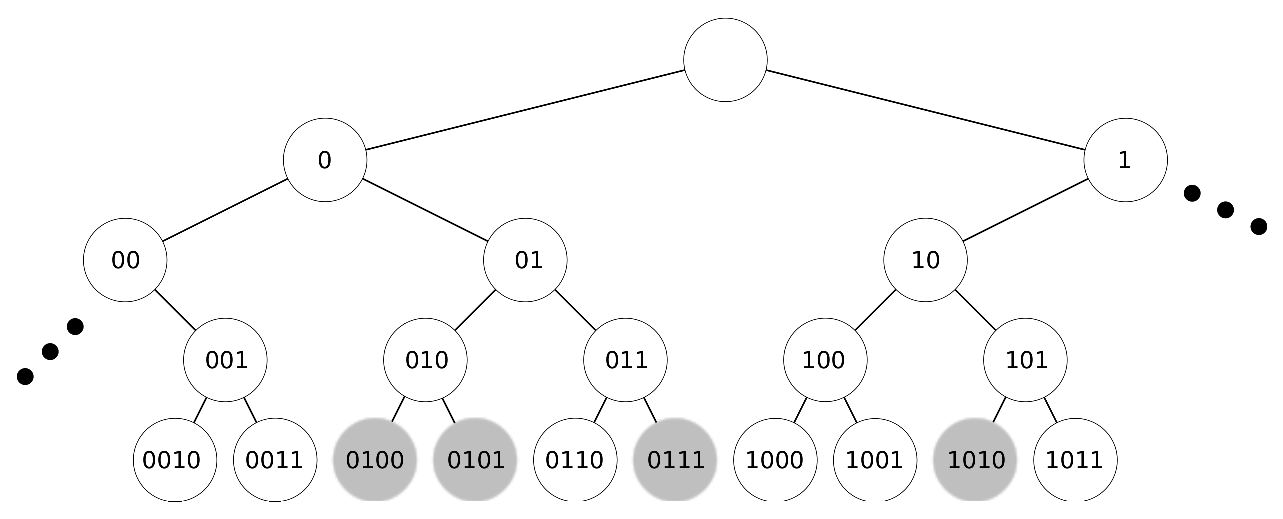
\includegraphics[width=5in]{Chapter_3_Figures/query_tree.eps}
\caption{Query tree singulation for a $4$ bit tag ID space.}
\label{Figure: query_tree.eps}
\end{figure}
\begin{figure}
\centering
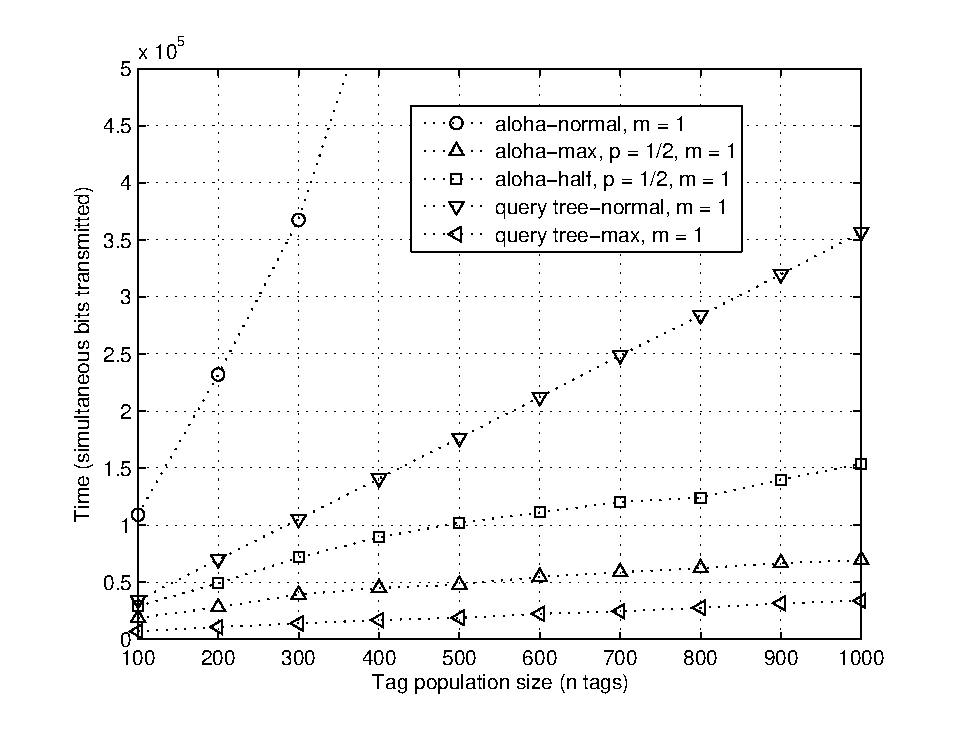
\includegraphics[width=5in]{Chapter_3_Figures/sta_read_all.eps}
\caption{Number of simultaneous bits transmitted for the static case. $m=1$.}
\label{Figure: sta_read_all.eps}
\end{figure}
\clearpage

\begin{figure}
\centering
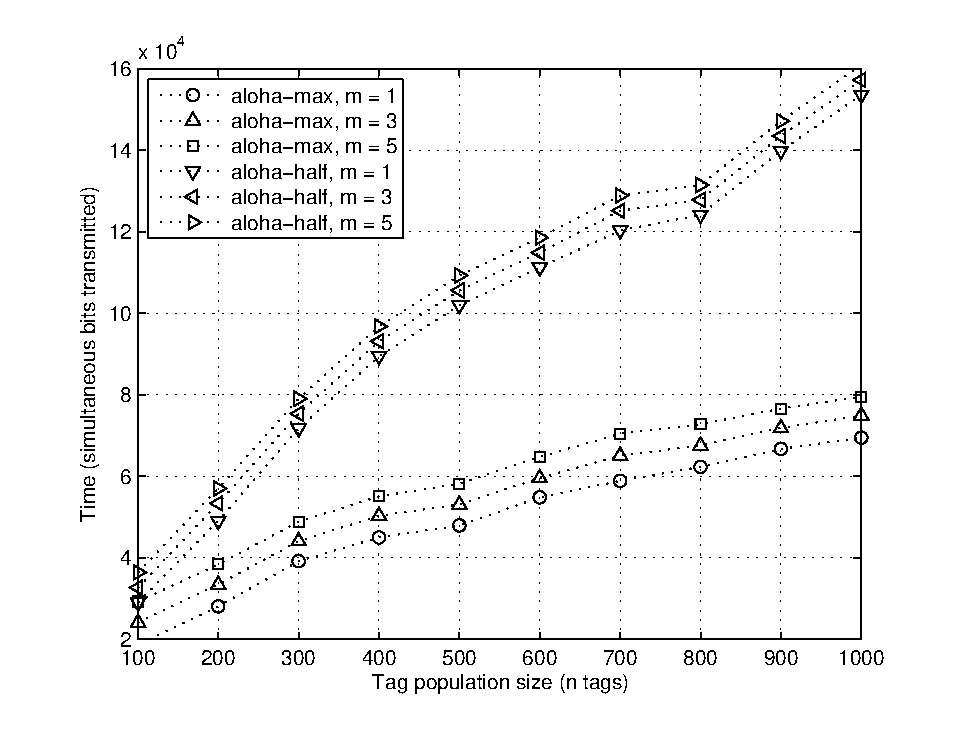
\includegraphics[width=5in]{Chapter_3_Figures/sta_read_aloha_max_aloha_half.eps}
\caption{Number of simultaneous bits transmitted for the static case. Aloha-based algorithms.}
\label{Figure: sta_read_aloha_max_aloha_half.eps}
\end{figure}
\begin{figure}
\centering
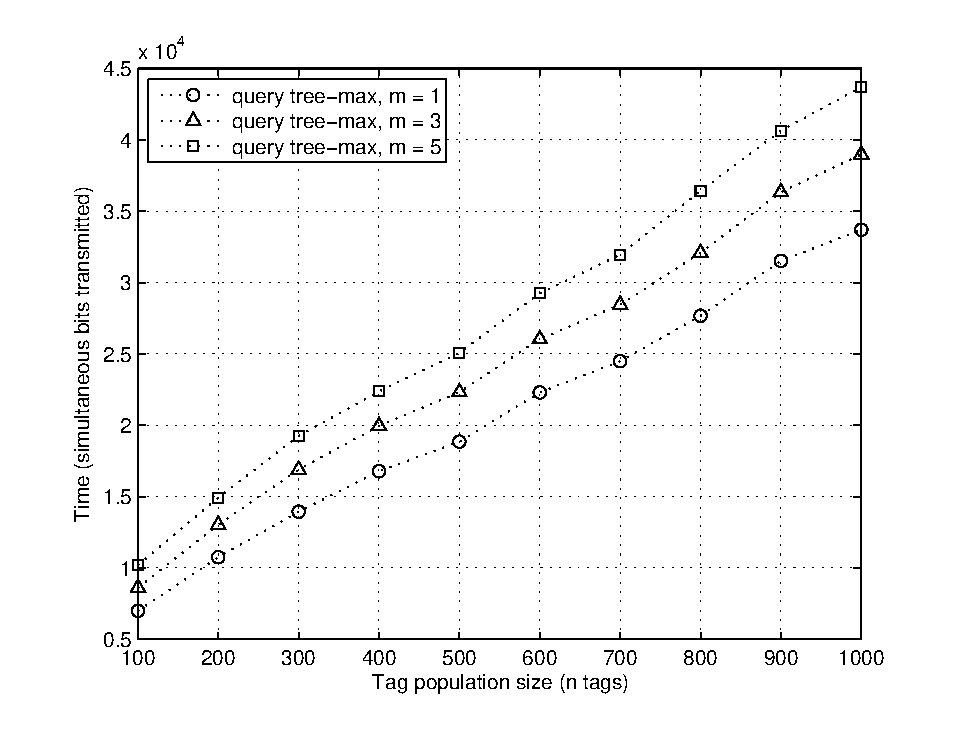
\includegraphics[width=5in]{Chapter_3_Figures/sta_read_qt_max.eps}
\caption{Number of simultaneous bits transmitted for the static case. Query tree-based algorithms.}
\label{Figure: sta_read_qt_max.eps}
\end{figure}
\clearpage

\begin{figure}
\centering
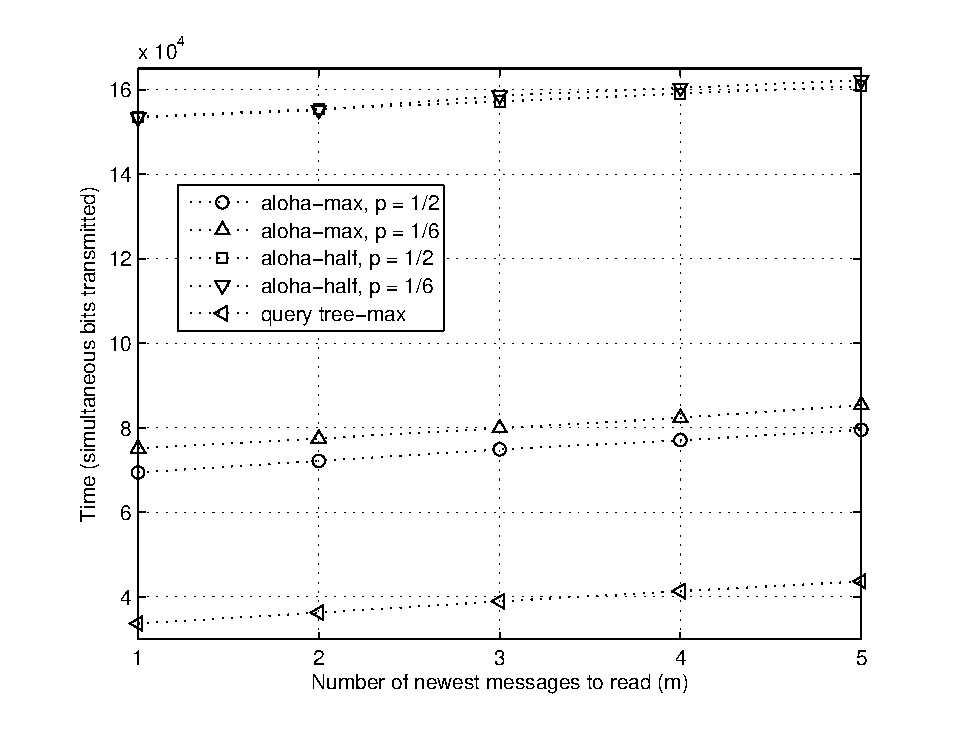
\includegraphics[width=5in]{Chapter_3_Figures/sta_read_increasing_m.eps}
\caption{Number of simultaneous bits transmitted for the static case. $n = 1000$ tags and increasing $m$.}
\label{Figure: sta_read_increasing_m.eps}
\end{figure}
\begin{figure}
\centering
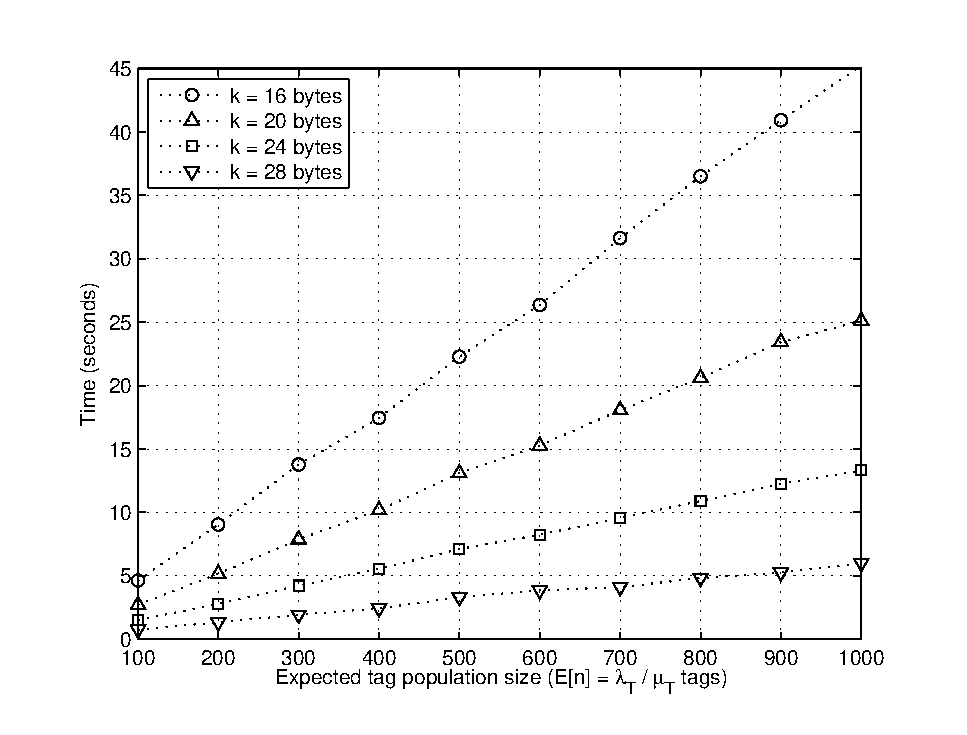
\includegraphics[width=5in]{Chapter_3_Figures/decay_lambda_I_0.2.eps}
\caption{Average measured message lifetime per byte. $p = \frac{1}{2}$ and $\lambda_I = 0.2$ arrivals per second.}
\label{Figure: decay_lambda_I_0.2.eps}
\end{figure}
\clearpage

\begin{figure}
\centering
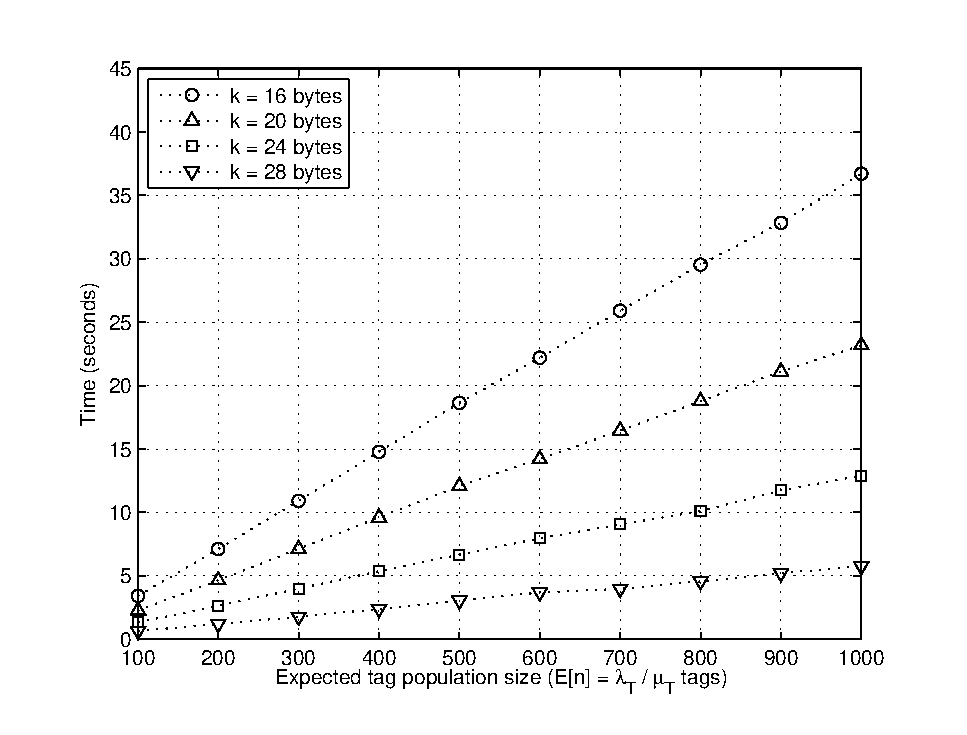
\includegraphics[width=5in]{Chapter_3_Figures/decay_lambda_I_0.6.eps}
\caption{Average measured message lifetime per byte. $p = \frac{1}{2}$ and $\lambda_I = 0.6$ arrivals per second.}
\label{Figure: decay_lambda_I_0.6.eps}
\end{figure}
\begin{figure}
\centering
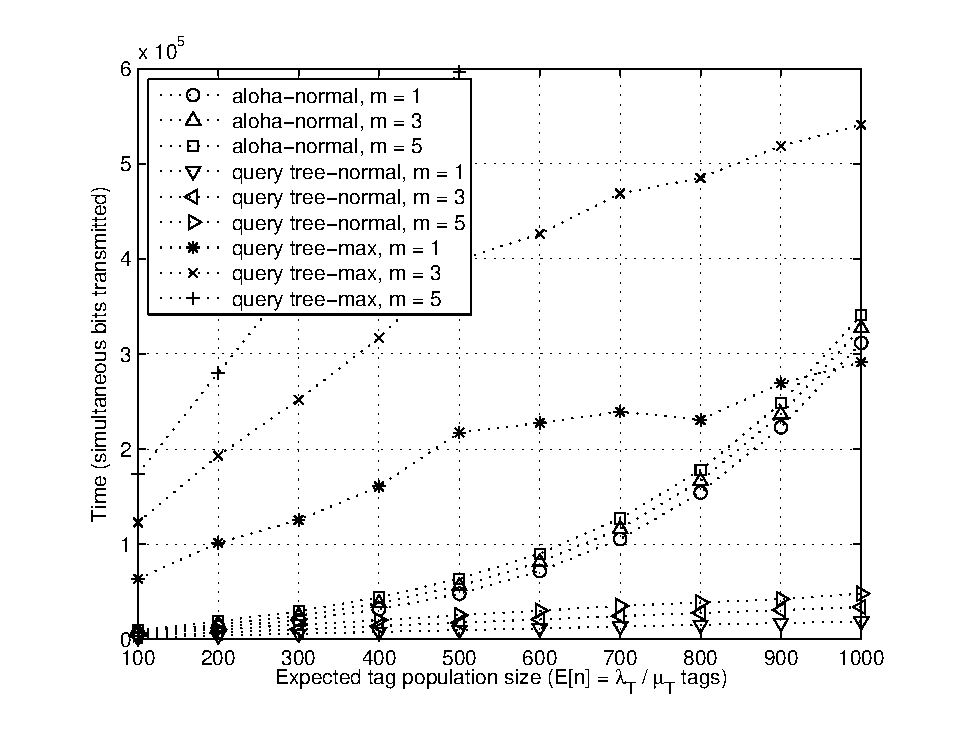
\includegraphics[width=5in]{Chapter_3_Figures/dyn_read_k_16.eps}
\caption{Average message access time per byte. $p= \frac{1}{2}$, $\lambda_I = 0.2$ arrivals per second, and $k = 16$ bytes.}
\label{Figure: dyn_read_k_16.eps}
\end{figure}
\clearpage

\begin{figure}
\centering
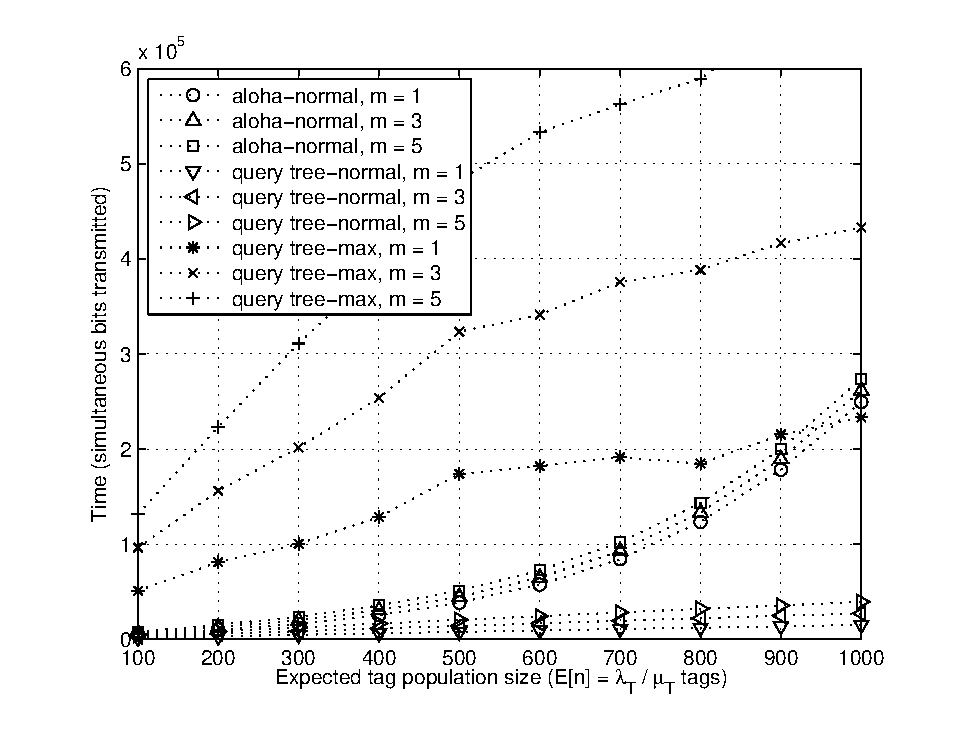
\includegraphics[width=5in]{Chapter_3_Figures/dyn_read_k_20.eps}
\caption{Average message access time per byte. $p= \frac{1}{2}$, $\lambda_I = 0.2$ arrivals per second, and $k = 20$ bytes.}
\label{Figure: dyn_read_k_20.eps}
\end{figure}
\begin{figure}
\centering
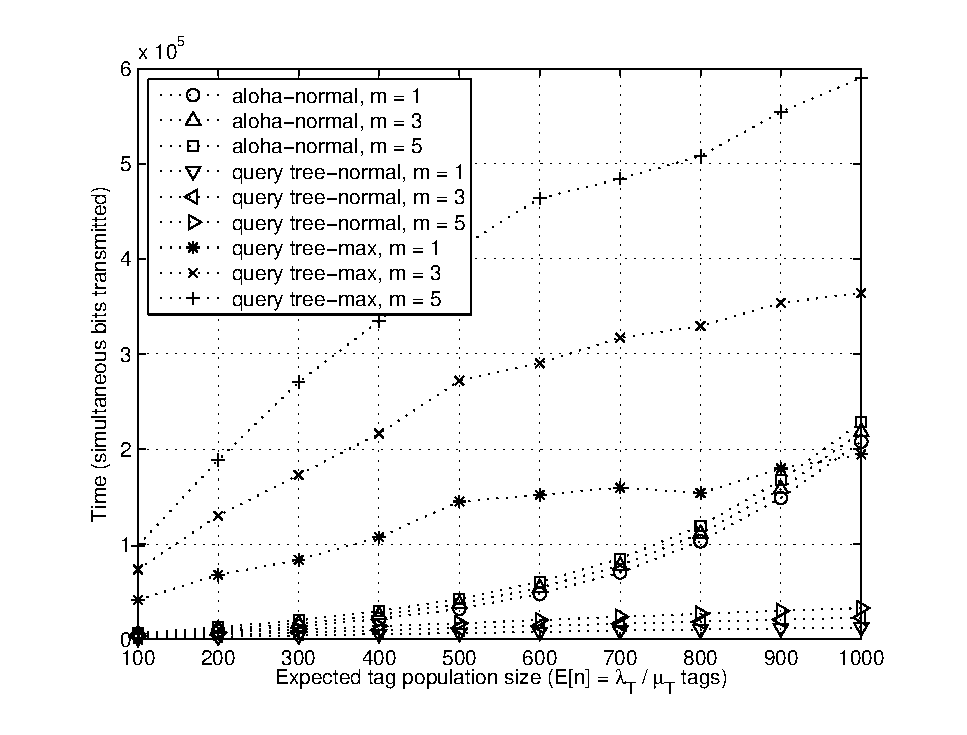
\includegraphics[width=5in]{Chapter_3_Figures/dyn_read_k_24.eps}
\caption{Average message access time per byte. $p= \frac{1}{2}$, $\lambda_I = 0.2$ arrivals per second, and $k = 24$ bytes.}
\label{Figure: dyn_read_k_24.eps}
\end{figure}
\clearpage

\begin{figure}
\centering
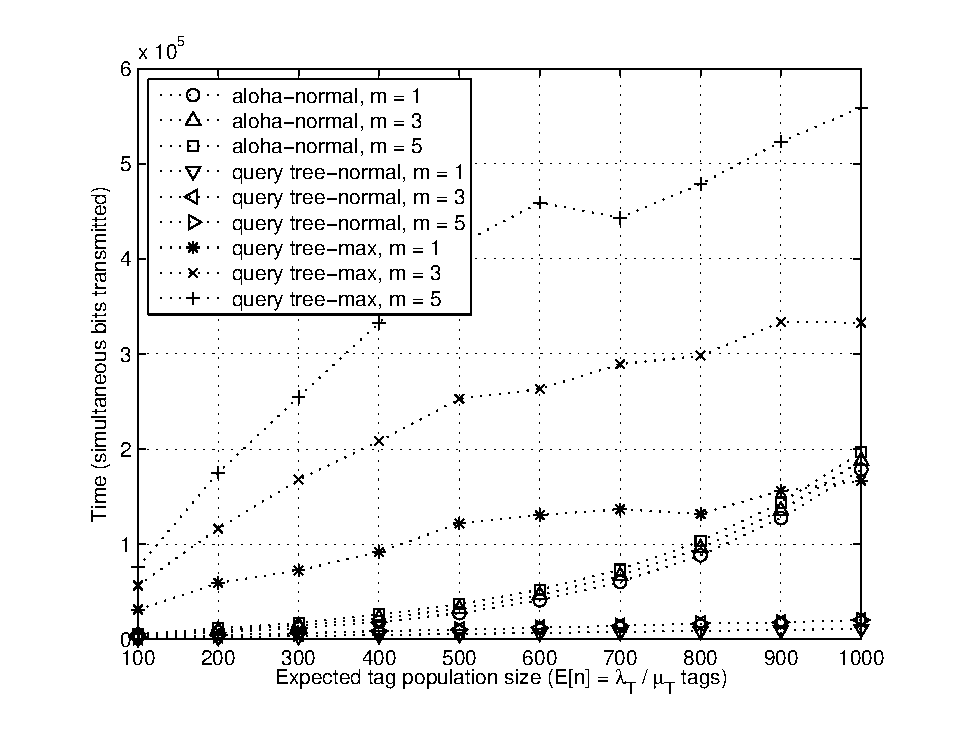
\includegraphics[width=5in]{Chapter_3_Figures/dyn_read_k_28.eps}
\caption{Average message access time per byte. $p= \frac{1}{2}$, $\lambda_I = 0.2$ arrivals per second, and $k = 28$ bytes.}
\label{Figure: dyn_read_k_28.eps}
\end{figure}
\begin{figure}
\centering
\includegraphics[height=5in, viewport=50 25 600 800, clip]{Chapter_3_Figures/Tag_Board_Figure.eps}
\caption{RFID tag board.}
\label{Figure: Tag_Board_Figure.eps}
\end{figure}
\clearpage

\begin{figure}
\centering
\includegraphics[width=5in, viewport=150 350 550 550, clip]{Chapter_3_Figures/Experiment_Setup.eps}
\caption{Experiment setup.}
\label{Figure: Experiment_Setup.eps}
\end{figure}
\clearpage

\begin{figure}
\centering
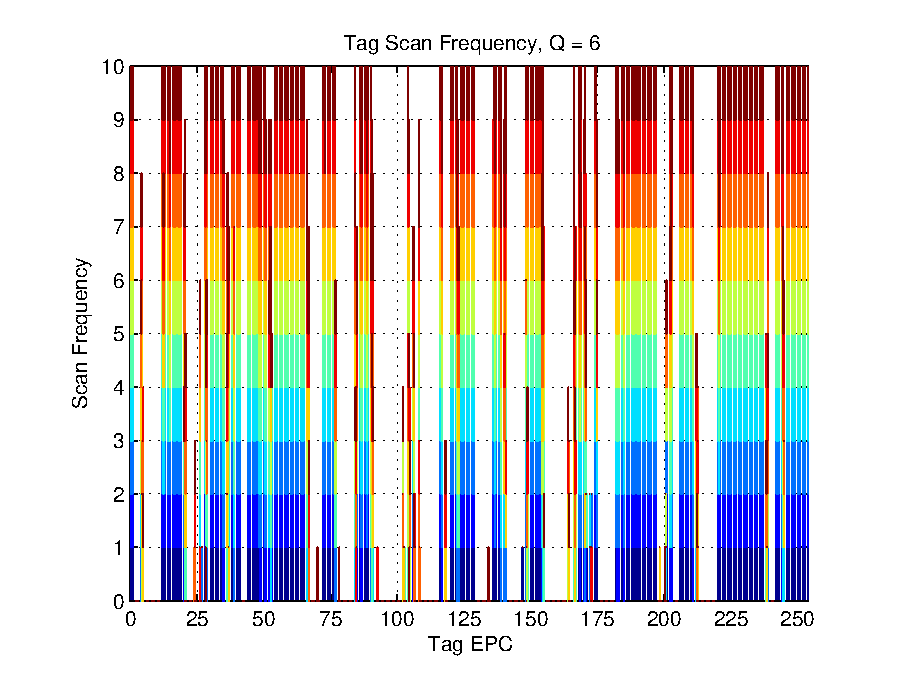
\includegraphics[width=5in]{Chapter_3_Figures/EPCList_Q06.eps}
\caption{Tag scan frequency. $F \in \{12, 20, 28\}$, $S \in \{4, 8, 16\}$, and $Q = 6$.}
\label{Figure: EPCList_Q06.eps}
\end{figure}
\begin{figure}
\centering
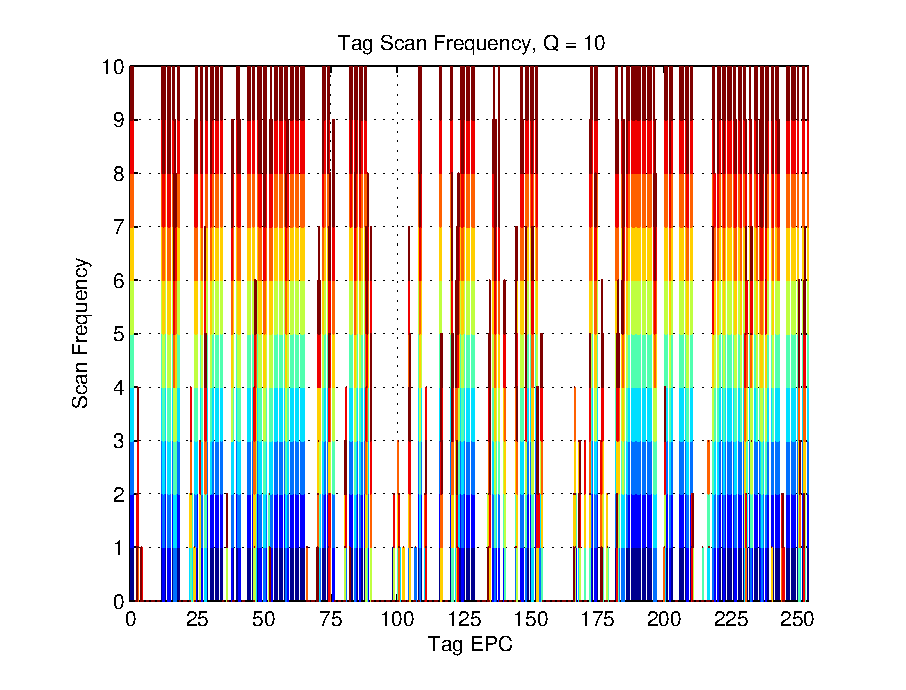
\includegraphics[width =5in]{Chapter_3_Figures/EPCList_Q10.eps}
\caption{Tag scan frequency. $F \in \{12, 20, 28\}$, $S \in \{4, 8, 16\}$, and $Q = 10$.}
\label{Figure: EPCList_Q10.eps}
\end{figure}
\clearpage

\begin{figure}
\centering
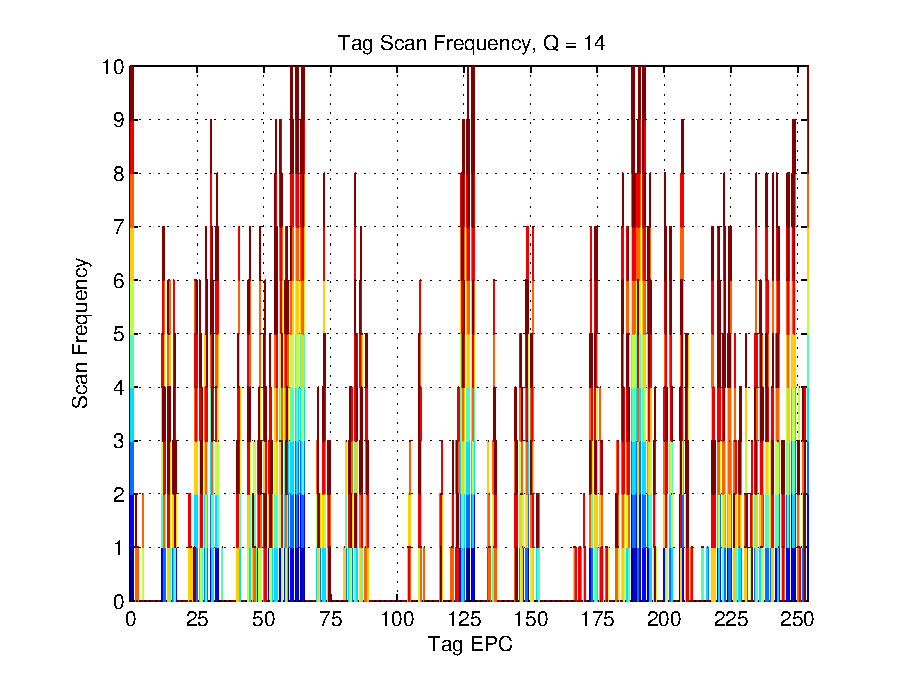
\includegraphics[width=5in]{Chapter_3_Figures/EPCList_Q14.eps}
\caption{Tag scan frequency. $F \in \{12, 20, 28\}$, $S \in \{4, 8, 16\}$, and $Q = 14$.}
\label{Figure: EPCList_Q14.eps}
\end{figure}
\begin{figure}
\centering
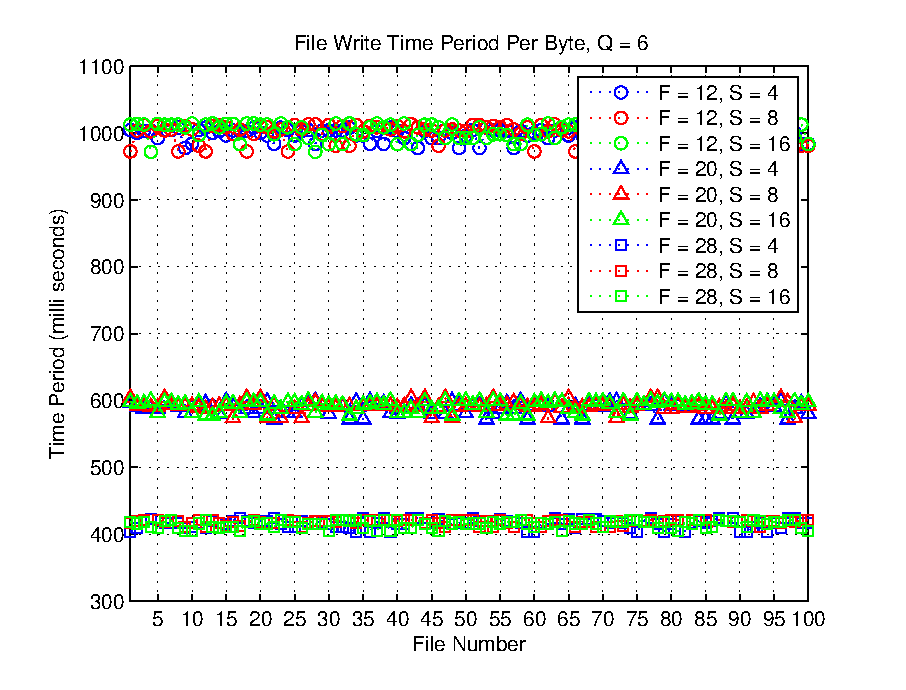
\includegraphics[width=5in]{Chapter_3_Figures/Write_Time_Q06.eps}
\caption{File write time period per byte. $F \in \{12, 20, 28\}$, $S \in \{4, 8, 16\}$, and $Q = 6$.}
\label{Figure: Write_Time_Q06.eps}
\end{figure}
\clearpage

\begin{figure}
\centering
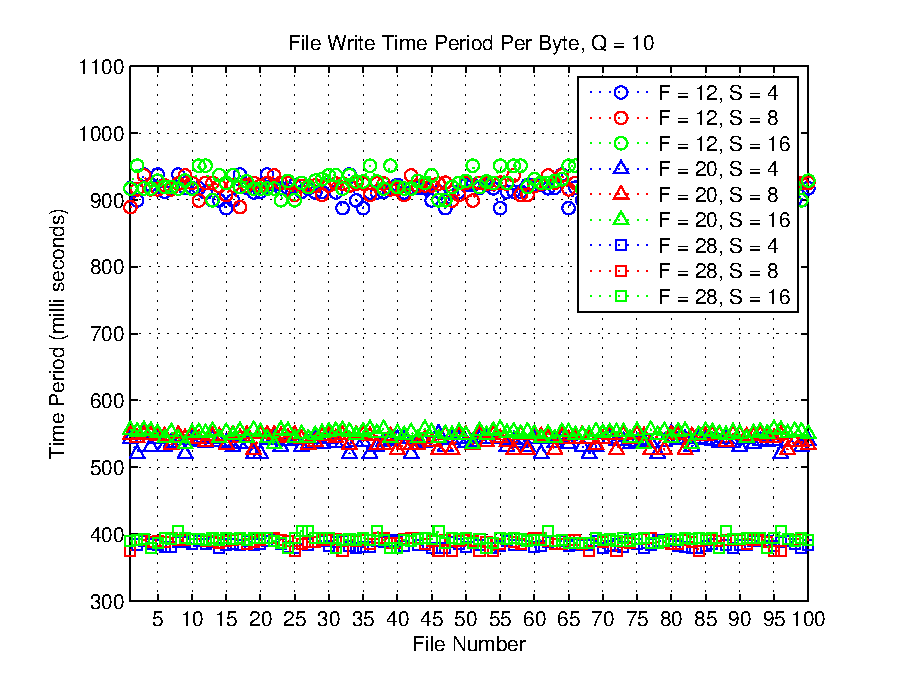
\includegraphics[width =5in]{Chapter_3_Figures/Write_Time_Q10.eps}
\caption{File write time period per byte. $F \in \{12, 20, 28\}$, $S \in \{4, 8, 16\}$, and $Q = 10$.}
\label{Figure: Write_Time_Q10.eps}
\end{figure}
\begin{figure}
\centering
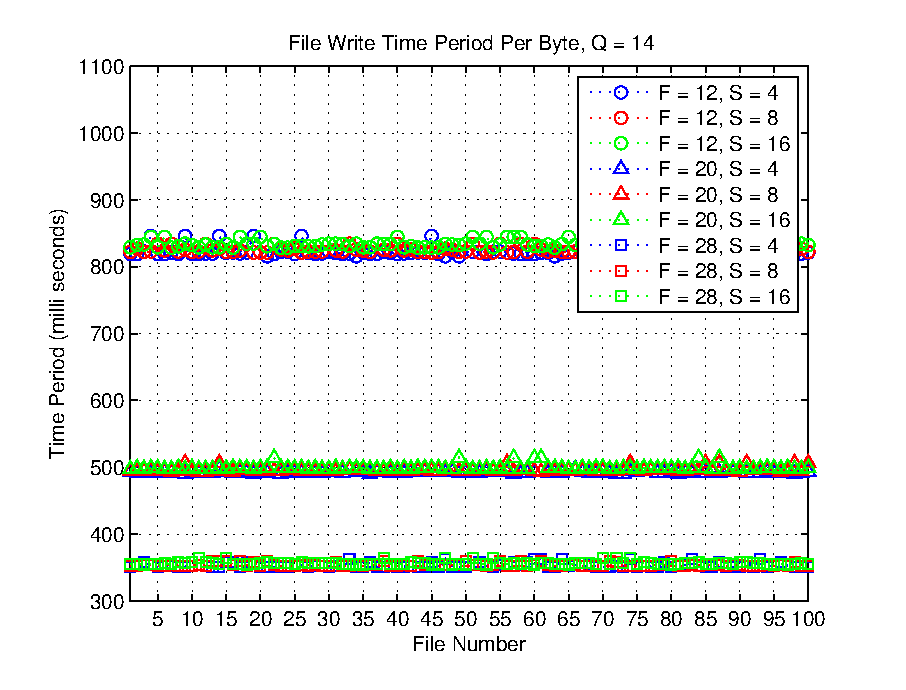
\includegraphics[width=5in]{Chapter_3_Figures/Write_Time_Q14.eps}
\caption{File write time period per byte. $F \in \{12, 20, 28\}$, $S \in \{4, 8, 16\}$, and $Q = 14$.}
\label{Figure: Write_Time_Q14.eps}
\end{figure}
\clearpage

\begin{figure}
\centering
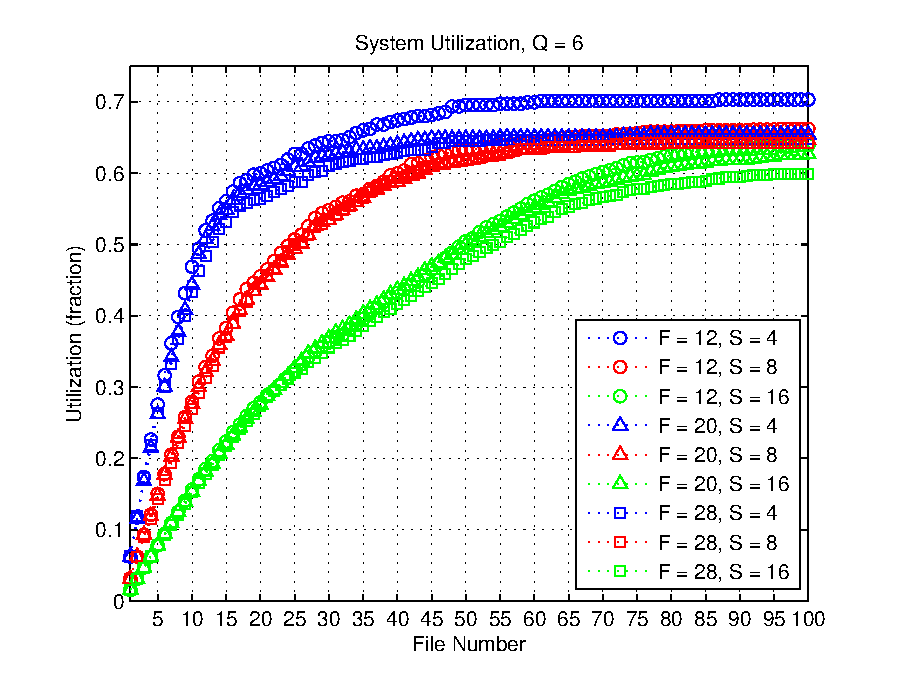
\includegraphics[width=5in]{Chapter_3_Figures/Utilization_Q06.eps}
\caption{System utilization. $F \in \{12, 20, 28\}$, $S \in \{4, 8, 16\}$, and $Q = 6$.}
\label{Figure: Utilization_Q06.eps}
\end{figure}
\begin{figure}
\centering
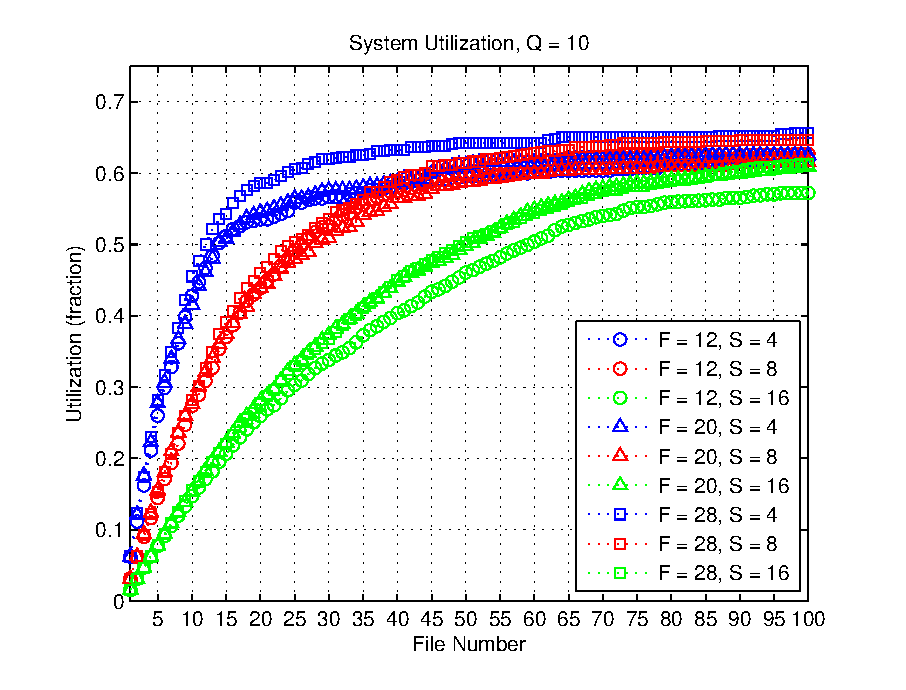
\includegraphics[width =5in]{Chapter_3_Figures/Utilization_Q10.eps}
\caption{System utilization. $F \in \{12, 20, 28\}$, $S \in \{4, 8, 16\}$, and $Q = 10$.}
\label{Figure: Utilization_Q10.eps}
\end{figure}
\clearpage

\begin{figure}
\centering
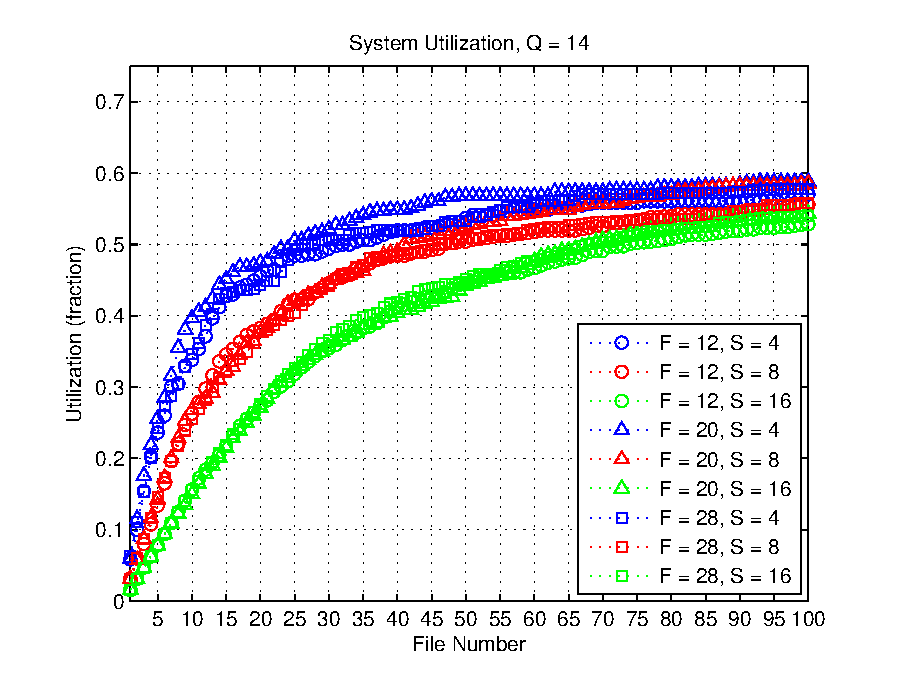
\includegraphics[width=5in]{Chapter_3_Figures/Utilization_Q14.eps}
\caption{System utilization. $F \in \{12, 20, 28\}$, $S \in \{4, 8, 16\}$, and $Q = 14$.}
\label{Figure: Utilization_Q14.eps}
\end{figure}
\begin{figure}
\centering
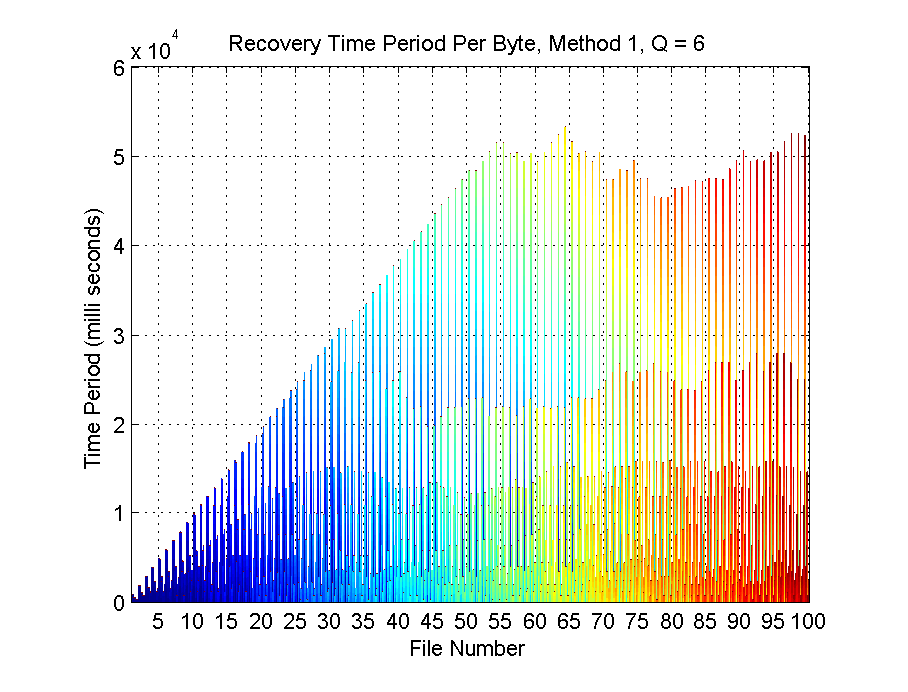
\includegraphics[width=5in]{Chapter_3_Figures/Recovery_Time_Q06.eps}
\caption{Recovery time period per byte. $F \in \{12, 20, 28\}$, $S \in \{4, 8, 16\}$, and $Q = 6$.}
\label{Figure: Recovery_Time_Q06.eps}
\end{figure}
\clearpage

\begin{figure}
\centering
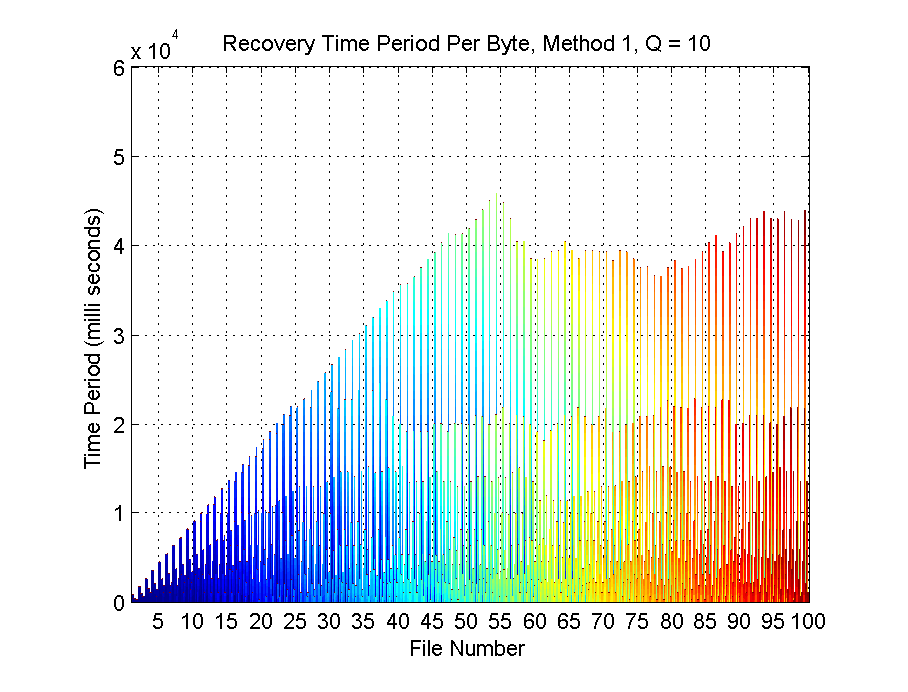
\includegraphics[width =5in]{Chapter_3_Figures/Recovery_Time_Q10.eps}
\caption{Recovery time period per byte. $F \in \{12, 20, 28\}$, $S \in \{4, 8, 16\}$, and $Q = 10$.}
\label{Figure: Recovery_Time_Q10.eps}
\end{figure}
\begin{figure}
\centering
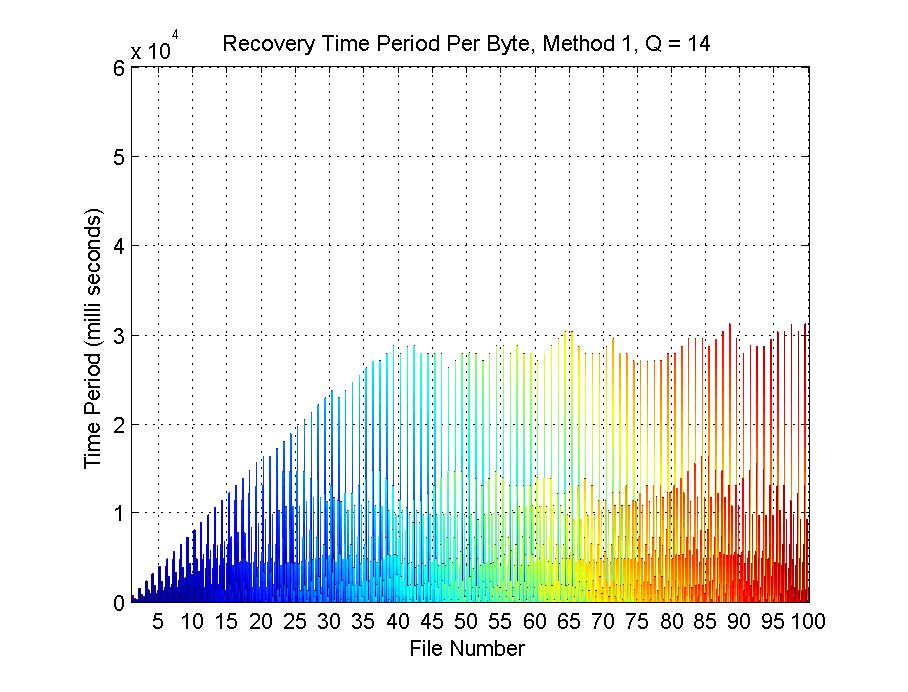
\includegraphics[width=5in]{Chapter_3_Figures/Recovery_Time_Q14.eps}
\caption{Recovery time period per byte. $F \in \{12, 20, 28\}$, $S \in \{4, 8, 16\}$, and $Q = 14$.}
\label{Figure: Recovery_Time_Q14.eps}
\end{figure}
\clearpage

\begin{figure}
\centering
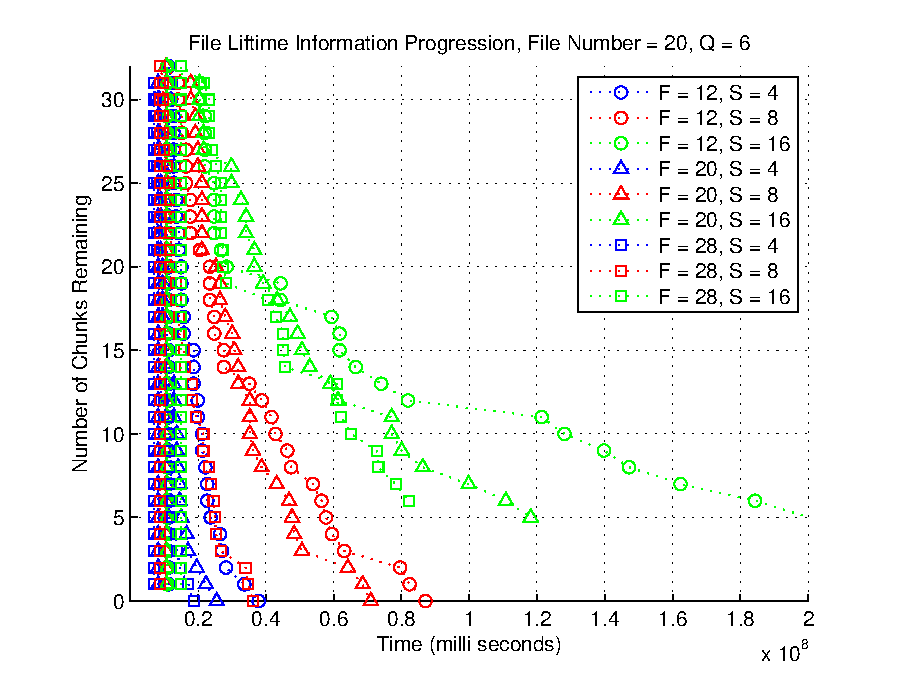
\includegraphics[width=5in]{Chapter_3_Figures/Lifetime_File20_Q06.eps}
\caption{File lifetime information progression. File number $= 20$, $F \in \{12, 20, 28\}$, $S \in \{4, 8, 16\}$, and $Q = 6$.}
\label{Figure: Lifetime_File20_Q06.eps}
\end{figure}
\begin{figure}
\centering
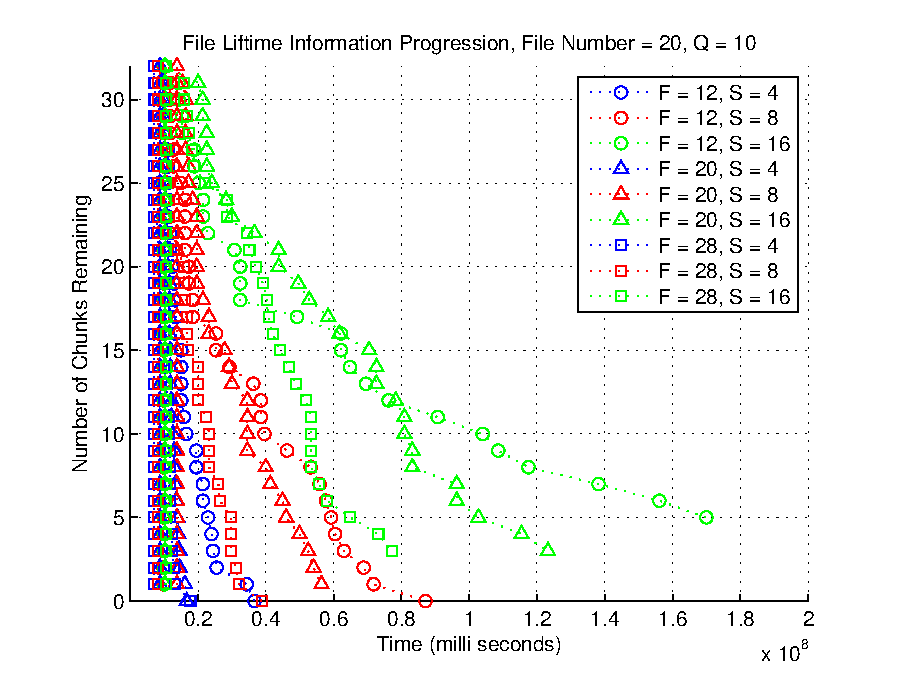
\includegraphics[width =5in]{Chapter_3_Figures/Lifetime_File20_Q10.eps}
\caption{File lifetime information progression. File number $= 20$, $F \in \{12, 20, 28\}$, $S \in \{4, 8, 16\}$, and $Q = 10$.}
\label{Figure: Lifetime_File20_Q10.eps}
\end{figure}
\clearpage

\begin{figure}
\centering
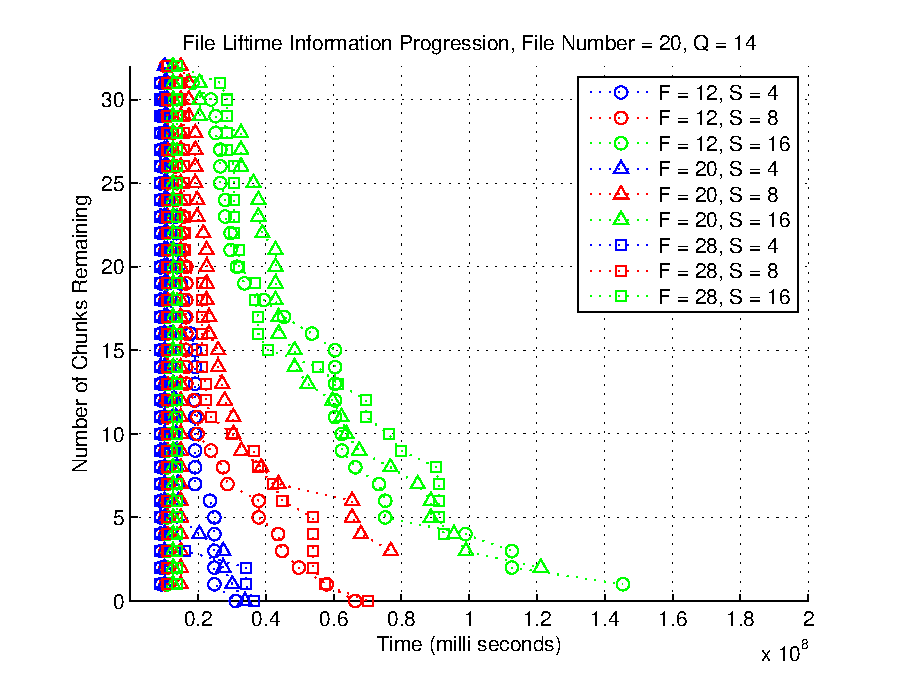
\includegraphics[width=5in]{Chapter_3_Figures/Lifetime_File20_Q14.eps}
\caption{File lifetime information progression. File number $= 20$, $F \in \{12, 20, 28\}$, $S \in \{4, 8, 16\}$, and $Q = 14$.}
\label{Figure: Lifetime_File20_Q14.eps}
\end{figure}
\begin{figure}
\centering
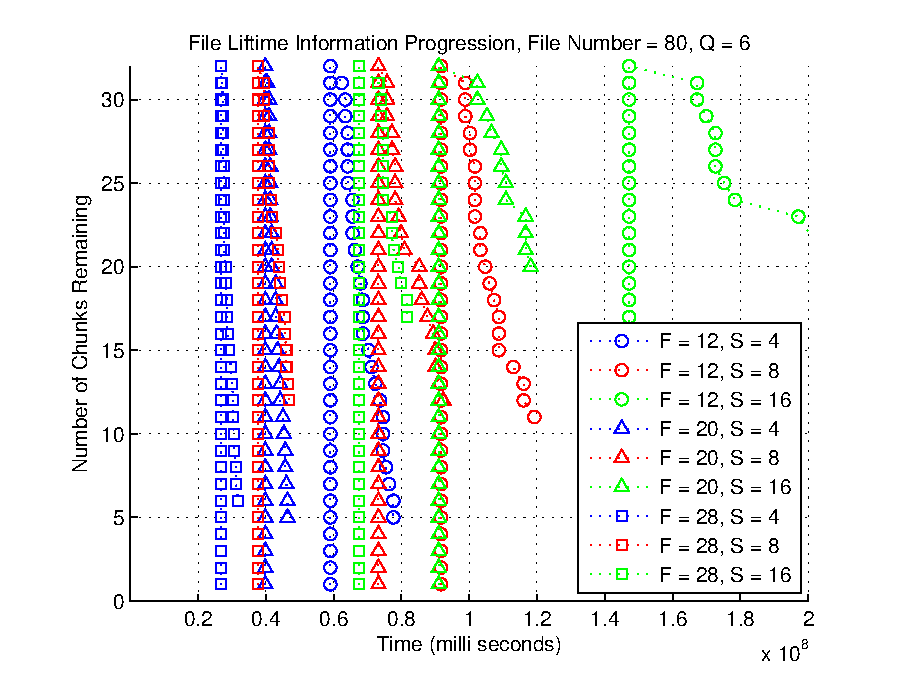
\includegraphics[width=5in]{Chapter_3_Figures/Lifetime_File80_Q06.eps}
\caption{File lifetime information progression. File number $= 80$, $F \in \{12, 20, 28\}$, $S \in \{4, 8, 16\}$, and $Q = 6$.}
\label{Figure: Lifetime_File80_Q06.eps}
\end{figure}
\clearpage

\begin{figure}
\centering
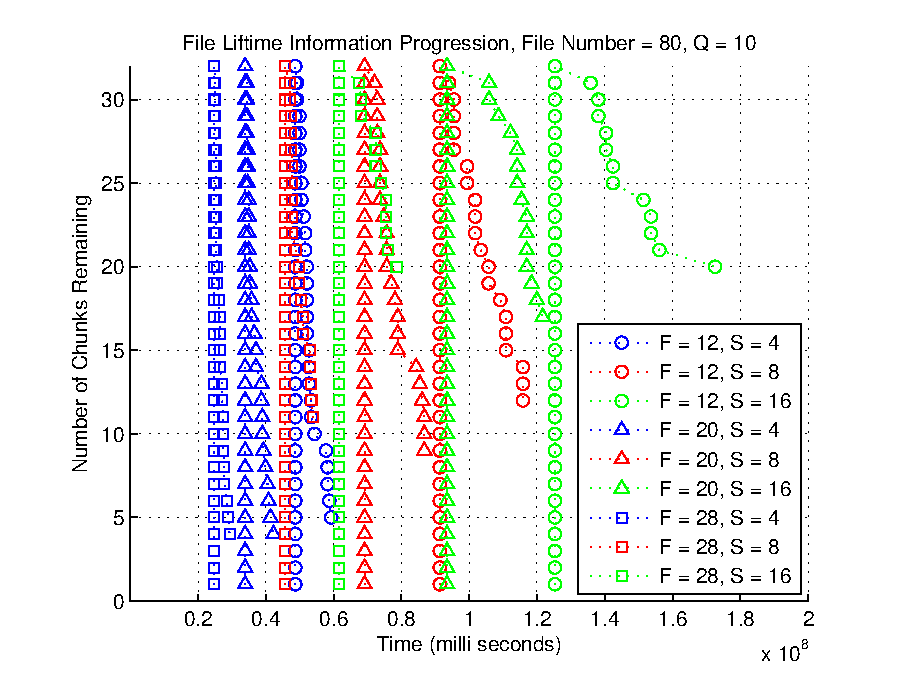
\includegraphics[width =5in]{Chapter_3_Figures/Lifetime_File80_Q10.eps}
\caption{File lifetime information progression. File number $= 80$, $F \in \{12, 20, 28\}$, $S \in \{4, 8, 16\}$, and $Q = 10$.}
\label{Figure: Lifetime_File80_Q10.eps}
\end{figure}
\begin{figure}
\centering
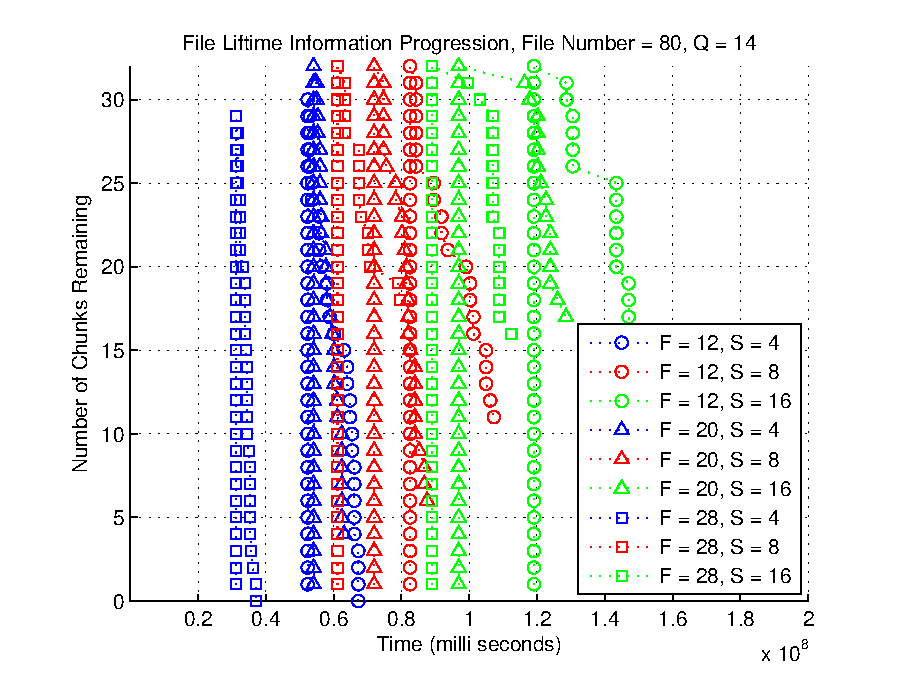
\includegraphics[width=5in]{Chapter_3_Figures/Lifetime_File80_Q14.eps}
\caption{File lifetime information progression. File number $= 80$, $F \in \{12, 20, 28\}$, $S \in \{4, 8, 16\}$, and $Q = 14$.}
\label{Figure: Lifetime_File80_Q14.eps}
\end{figure}
\clearpage

\begin{table}
\caption{Choice of $N$.}
\label{Table: Choice of $N$.}
\begin{center} 
\begin{tabular}{| c || c | c | c | c | c |} 
\hline
$\hat{n} \in $ & $\left[1,9\right]$ & $ \left[10,27\right]$ & $ \left[28,56\right]$ & $\ \left[57,129\right]$ & $ \left[130,\infty\right)$ \\
\hline
$N$ & $16$ & $32$ & $64$ & $128$ & $256$\\
\hline
\end{tabular}
\end{center}
\end{table}

\begin{table}
\caption{Aloha-based communications.}
\label{Table: Aloha-based communications.}
\begin{center}
\begin{tabular}{| c | l | }
\hline
\multirow{4}{*}{Aloha-normal}
 & $I \stackrel{N}{\xrightarrow{\hspace*{1.5cm}}} \{T_j\}_{j=1}^n$\\ 
 & \\
 & For $j \in \{1, \ldots, n\}$, \\
 & in $k_{T_j}^{th}$ time slot: $I \stackrel{ID_j, ts_j}{\xleftarrow{\hspace*{1.5cm}}} T_j, $ \\
 \hline
\multirow{4}{*}{Aloha-max}
 & $I \stackrel{N, ts_{largest}}{\xrightarrow{\hspace*{1.5cm}}} \{T_j\}_{j=1}^n$ \\ 
 & \\
 &  For $j \in \{1, \ldots, n\}$, if $ts_j > ts_{largest}$, \\
 & then in $k_{T_j}^{th}$ time slot: $I \stackrel{ID_j, ts_j}{\xleftarrow{\hspace*{1.5cm}}} T_j$ \\
 \hline
\multirow{4}{*}{Aloha-half}
 & $I \stackrel{N, ts_{median}}{\xrightarrow{\hspace*{1.5cm}}} \{T_j\}_{j=1}^n$ \\ 
 & \\
 &  For $j \in \{1, \ldots, n\}$, if $ts_j > ts_{median}$, \\
 & then in $k_{T_j}^{th}$ time slot: $I \stackrel{ID_j, ts_j}{\xleftarrow{\hspace*{1.5cm}}} T_j$ \\
 \hline
 \end{tabular}
\end{center}
\end{table}

\begin{table}
\caption{Simultaneous bits transmitted in each round.}
\label{Table: Simultaneous bits transmitted in each round.}
\begin{center}
\begin{tabular}{| c | l | }
\hline
\multicolumn{2}{|c|}{\textbf{Aloha-based}} \\ 
\hline
\multirow{2}{*}{Aloha-normal}
 & Interrogator query: $3$ bits \\ 
 & Tag response: $N \left(96 + 17\right)$ bits\\
 \hline
\multirow{2}{*}{Aloha-max}
 & Interrogator query: $3 + 17$ bits \\ 
 & Tag response: $N \left(96 + 17\right)$ bits\\
 \hline
\multirow{2}{*}{Aloha-half}
 & Interrogator query: $3 + 17$ bits \\ 
 & Tag response: $N \left(96 + 17\right)$ bits\\
 \hline 
 \multicolumn{2}{|c|}{\textbf{Query Tree-based}} \\ 
\hline
\multirow{3}{*}{Query tree-normal}
 & Interrogator query: length(bit string) bits \\ 
 & Tag response: $96 + 17$ bits\\
 \hline
\multirow{3}{*}{Query tree-max}
 & Interrogator query: length(bit string) + $17$ bits \\ 
 & Tag response: $96 + 17$ bits\\
 \hline
 \end{tabular}
\end{center}
\end{table}

\begin{table}
\caption{Performance tradeoffs in the dynamic case.}
\label{Table: Performance tradeoffs in the dynamic case.}
\begin{center}
\begin{tabular}{|c|c|c|c|} 
\hline
\multirow{2}{*}{$k$} & \multirow{2}{*}{\textbf{Coding Buffer}} & \multicolumn{2}{|c|}{\textbf{Performance Metrics (per byte)}} \\ \cline{3-4}
&& Message Lifetime & Message Access Time\\ 
\hline
Small & Large & Long & Long \\
\hline
Large & Small & Short & Short\\
\hline
\end{tabular}
\end{center}
\end{table}
